\documentclass{report}

%%%%%%%%%%%%%%%%%%%%%%%%%%%%%%%%%
% PACKAGE IMPORTS
%%%%%%%%%%%%%%%%%%%%%%%%%%%%%%%%%


\usepackage[tmargin=2cm,rmargin=1in,lmargin=1in,margin=0.85in,bmargin=2cm,footskip=.2in]{geometry}
\usepackage{amsmath,amsfonts,amsthm,amssymb,mathtools}
\usepackage[varbb]{newpxmath}
\usepackage{xfrac}
\usepackage[makeroom]{cancel}
\usepackage{mathtools}
\usepackage{bookmark}
\usepackage{enumitem}
\usepackage{hyperref,theoremref}
\usepackage{graphicx}
\graphicspath{ {./img} }
\hypersetup{
	pdftitle={Assignment},
	colorlinks=true, linkcolor=doc!90,
	bookmarksnumbered=true,
	bookmarksopen=true
}
\usepackage[most,many,breakable]{tcolorbox}
\usepackage{xcolor}
\usepackage{varwidth}
\usepackage{varwidth}
\usepackage{etoolbox}
%\usepackage{authblk}
\usepackage{nameref}
\usepackage{multicol,array}
\usepackage{tikz-cd}
\usepackage[ruled,vlined,linesnumbered]{algorithm2e}
\usepackage{comment} % enables the use of multi-line comments (\ifx \fi) 
\usepackage{import}
\usepackage{xifthen}
\usepackage{pdfpages}
\usepackage{transparent}

\newcommand\mycommfont[1]{\footnotesize\ttfamily\textcolor{blue}{#1}}
\SetCommentSty{mycommfont}
\newcommand{\incfig}[1]{%
    \def\svgwidth{\columnwidth}
    \import{./figures/}{#1.pdf_tex}
}

\usepackage{tikzsymbols}
\renewcommand\qedsymbol{$\Laughey$}


%\usepackage{import}
%\usepackage{xifthen}
%\usepackage{pdfpages}
%\usepackage{transparent}


%%%%%%%%%%%%%%%%%%%%%%%%%%%%%%
% SELF MADE COLORS
%%%%%%%%%%%%%%%%%%%%%%%%%%%%%%



\definecolor{myg}{RGB}{56, 140, 70}
\definecolor{myb}{RGB}{45, 111, 177}
\definecolor{myr}{RGB}{199, 68, 64}
\definecolor{mytheorembg}{HTML}{F2F2F9}
\definecolor{mytheoremfr}{HTML}{00007B}
\definecolor{mylenmabg}{HTML}{FFFAF8}
\definecolor{mylenmafr}{HTML}{983b0f}
\definecolor{mypropbg}{HTML}{f2fbfc}
\definecolor{mypropfr}{HTML}{191971}
\definecolor{myexamplebg}{HTML}{F2FBF8}
\definecolor{myexamplefr}{HTML}{88D6D1}
\definecolor{myexampleti}{HTML}{2A7F7F}
\definecolor{mydefinitbg}{HTML}{E5E5FF}
\definecolor{mydefinitfr}{HTML}{3F3FA3}
\definecolor{notesgreen}{RGB}{0,162,0}
\definecolor{myp}{RGB}{197, 92, 212}
\definecolor{mygr}{HTML}{2C3338}
\definecolor{myred}{RGB}{127,0,0}
\definecolor{myyellow}{RGB}{169,121,69}
\definecolor{myexercisebg}{HTML}{F2FBF8}
\definecolor{myexercisefg}{HTML}{88D6D1}


%%%%%%%%%%%%%%%%%%%%%%%%%%%%
% TCOLORBOX SETUPS
%%%%%%%%%%%%%%%%%%%%%%%%%%%%

\setlength{\parindent}{1cm}
%================================
% THEOREM BOX
%================================

\tcbuselibrary{theorems,skins,hooks}
\newtcbtheorem[number within=section]{Theorem}{Theorem}
{%
	enhanced,
	breakable,
	colback = mytheorembg,
	frame hidden,
	boxrule = 0sp,
	borderline west = {2pt}{0pt}{mytheoremfr},
	sharp corners,
	detach title,
	before upper = \tcbtitle\par\smallskip,
	coltitle = mytheoremfr,
	fonttitle = \bfseries\sffamily,
	description font = \mdseries,
	separator sign none,
	segmentation style={solid, mytheoremfr},
}
{th}

\tcbuselibrary{theorems,skins,hooks}
\newtcbtheorem[number within=chapter]{theorem}{Theorem}
{%
	enhanced,
	breakable,
	colback = mytheorembg,
	frame hidden,
	boxrule = 0sp,
	borderline west = {2pt}{0pt}{mytheoremfr},
	sharp corners,
	detach title,
	before upper = \tcbtitle\par\smallskip,
	coltitle = mytheoremfr,
	fonttitle = \bfseries\sffamily,
	description font = \mdseries,
	separator sign none,
	segmentation style={solid, mytheoremfr},
}
{th}


\tcbuselibrary{theorems,skins,hooks}
\newtcolorbox{Theoremcon}
{%
	enhanced
	,breakable
	,colback = mytheorembg
	,frame hidden
	,boxrule = 0sp
	,borderline west = {2pt}{0pt}{mytheoremfr}
	,sharp corners
	,description font = \mdseries
	,separator sign none
}

%================================
% Corollery
%================================
\tcbuselibrary{theorems,skins,hooks}
\newtcbtheorem[number within=section]{Corollary}{Corollary}
{%
	enhanced
	,breakable
	,colback = myp!10
	,frame hidden
	,boxrule = 0sp
	,borderline west = {2pt}{0pt}{myp!85!black}
	,sharp corners
	,detach title
	,before upper = \tcbtitle\par\smallskip
	,coltitle = myp!85!black
	,fonttitle = \bfseries\sffamily
	,description font = \mdseries
	,separator sign none
	,segmentation style={solid, myp!85!black}
}
{th}
\tcbuselibrary{theorems,skins,hooks}
\newtcbtheorem[number within=chapter]{corollary}{Corollary}
{%
	enhanced
	,breakable
	,colback = myp!10
	,frame hidden
	,boxrule = 0sp
	,borderline west = {2pt}{0pt}{myp!85!black}
	,sharp corners
	,detach title
	,before upper = \tcbtitle\par\smallskip
	,coltitle = myp!85!black
	,fonttitle = \bfseries\sffamily
	,description font = \mdseries
	,separator sign none
	,segmentation style={solid, myp!85!black}
}
{th}


%================================
% LENMA
%================================

\tcbuselibrary{theorems,skins,hooks}
\newtcbtheorem[number within=section]{Lenma}{Lenma}
{%
	enhanced,
	breakable,
	colback = mylenmabg,
	frame hidden,
	boxrule = 0sp,
	borderline west = {2pt}{0pt}{mylenmafr},
	sharp corners,
	detach title,
	before upper = \tcbtitle\par\smallskip,
	coltitle = mylenmafr,
	fonttitle = \bfseries\sffamily,
	description font = \mdseries,
	separator sign none,
	segmentation style={solid, mylenmafr},
}
{th}

\tcbuselibrary{theorems,skins,hooks}
\newtcbtheorem[number within=chapter]{lenma}{Lenma}
{%
	enhanced,
	breakable,
	colback = mylenmabg,
	frame hidden,
	boxrule = 0sp,
	borderline west = {2pt}{0pt}{mylenmafr},
	sharp corners,
	detach title,
	before upper = \tcbtitle\par\smallskip,
	coltitle = mylenmafr,
	fonttitle = \bfseries\sffamily,
	description font = \mdseries,
	separator sign none,
	segmentation style={solid, mylenmafr},
}
{th}


%================================
% PROPOSITION
%================================

\tcbuselibrary{theorems,skins,hooks}
\newtcbtheorem[number within=section]{Prop}{Proposition}
{%
	enhanced,
	breakable,
	colback = mypropbg,
	frame hidden,
	boxrule = 0sp,
	borderline west = {2pt}{0pt}{mypropfr},
	sharp corners,
	detach title,
	before upper = \tcbtitle\par\smallskip,
	coltitle = mypropfr,
	fonttitle = \bfseries\sffamily,
	description font = \mdseries,
	separator sign none,
	segmentation style={solid, mypropfr},
}
{th}

\tcbuselibrary{theorems,skins,hooks}
\newtcbtheorem[number within=chapter]{prop}{Proposition}
{%
	enhanced,
	breakable,
	colback = mypropbg,
	frame hidden,
	boxrule = 0sp,
	borderline west = {2pt}{0pt}{mypropfr},
	sharp corners,
	detach title,
	before upper = \tcbtitle\par\smallskip,
	coltitle = mypropfr,
	fonttitle = \bfseries\sffamily,
	description font = \mdseries,
	separator sign none,
	segmentation style={solid, mypropfr},
}
{th}


%================================
% CLAIM
%================================

\tcbuselibrary{theorems,skins,hooks}
\newtcbtheorem[number within=section]{claim}{Claim}
{%
	enhanced
	,breakable
	,colback = myg!10
	,frame hidden
	,boxrule = 0sp
	,borderline west = {2pt}{0pt}{myg}
	,sharp corners
	,detach title
	,before upper = \tcbtitle\par\smallskip
	,coltitle = myg!85!black
	,fonttitle = \bfseries\sffamily
	,description font = \mdseries
	,separator sign none
	,segmentation style={solid, myg!85!black}
}
{th}



%================================
% Exercise
%================================

\tcbuselibrary{theorems,skins,hooks}
\newtcbtheorem[number within=section]{Exercise}{Exercise}
{%
	enhanced,
	breakable,
	colback = myexercisebg,
	frame hidden,
	boxrule = 0sp,
	borderline west = {2pt}{0pt}{myexercisefg},
	sharp corners,
	detach title,
	before upper = \tcbtitle\par\smallskip,
	coltitle = myexercisefg,
	fonttitle = \bfseries\sffamily,
	description font = \mdseries,
	separator sign none,
	segmentation style={solid, myexercisefg},
}
{th}

\tcbuselibrary{theorems,skins,hooks}
\newtcbtheorem[number within=chapter]{exercise}{Exercise}
{%
	enhanced,
	breakable,
	colback = myexercisebg,
	frame hidden,
	boxrule = 0sp,
	borderline west = {2pt}{0pt}{myexercisefg},
	sharp corners,
	detach title,
	before upper = \tcbtitle\par\smallskip,
	coltitle = myexercisefg,
	fonttitle = \bfseries\sffamily,
	description font = \mdseries,
	separator sign none,
	segmentation style={solid, myexercisefg},
}
{th}

%================================
% EXAMPLE BOX
%================================

\newtcbtheorem[number within=section]{Example}{Example}
{%
	colback = myexamplebg
	,breakable
	,colframe = myexamplefr
	,coltitle = myexampleti
	,boxrule = 1pt
	,sharp corners
	,detach title
	,before upper=\tcbtitle\par\smallskip
	,fonttitle = \bfseries
	,description font = \mdseries
	,separator sign none
	,description delimiters parenthesis
}
{ex}

\newtcbtheorem[number within=chapter]{example}{Example}
{%
	colback = myexamplebg
	,breakable
	,colframe = myexamplefr
	,coltitle = myexampleti
	,boxrule = 1pt
	,sharp corners
	,detach title
	,before upper=\tcbtitle\par\smallskip
	,fonttitle = \bfseries
	,description font = \mdseries
	,separator sign none
	,description delimiters parenthesis
}
{ex}

%================================
% DEFINITION BOX
%================================

\newtcbtheorem[number within=section]{Definition}{Definition}{enhanced,
	before skip=2mm,after skip=2mm, colback=red!5,colframe=red!80!black,boxrule=0.5mm,
	attach boxed title to top left={xshift=1cm,yshift*=1mm-\tcboxedtitleheight}, varwidth boxed title*=-3cm,
	boxed title style={frame code={
					\path[fill=tcbcolback]
					([yshift=-1mm,xshift=-1mm]frame.north west)
					arc[start angle=0,end angle=180,radius=1mm]
					([yshift=-1mm,xshift=1mm]frame.north east)
					arc[start angle=180,end angle=0,radius=1mm];
					\path[left color=tcbcolback!60!black,right color=tcbcolback!60!black,
						middle color=tcbcolback!80!black]
					([xshift=-2mm]frame.north west) -- ([xshift=2mm]frame.north east)
					[rounded corners=1mm]-- ([xshift=1mm,yshift=-1mm]frame.north east)
					-- (frame.south east) -- (frame.south west)
					-- ([xshift=-1mm,yshift=-1mm]frame.north west)
					[sharp corners]-- cycle;
				},interior engine=empty,
		},
	fonttitle=\bfseries,
	title={#2},#1}{def}
\newtcbtheorem[number within=chapter]{definition}{Definition}{enhanced,
	before skip=2mm,after skip=2mm, colback=red!5,colframe=red!80!black,boxrule=0.5mm,
	attach boxed title to top left={xshift=1cm,yshift*=1mm-\tcboxedtitleheight}, varwidth boxed title*=-3cm,
	boxed title style={frame code={
					\path[fill=tcbcolback]
					([yshift=-1mm,xshift=-1mm]frame.north west)
					arc[start angle=0,end angle=180,radius=1mm]
					([yshift=-1mm,xshift=1mm]frame.north east)
					arc[start angle=180,end angle=0,radius=1mm];
					\path[left color=tcbcolback!60!black,right color=tcbcolback!60!black,
						middle color=tcbcolback!80!black]
					([xshift=-2mm]frame.north west) -- ([xshift=2mm]frame.north east)
					[rounded corners=1mm]-- ([xshift=1mm,yshift=-1mm]frame.north east)
					-- (frame.south east) -- (frame.south west)
					-- ([xshift=-1mm,yshift=-1mm]frame.north west)
					[sharp corners]-- cycle;
				},interior engine=empty,
		},
	fonttitle=\bfseries,
	title={#2},#1}{def}



%================================
% Solution BOX
%================================

\makeatletter
\newtcbtheorem{question}{Question}{enhanced,
	breakable,
	colback=white,
	colframe=myb!80!black,
	attach boxed title to top left={yshift*=-\tcboxedtitleheight},
	fonttitle=\bfseries,
	title={#2},
	boxed title size=title,
	boxed title style={%
			sharp corners,
			rounded corners=northwest,
			colback=tcbcolframe,
			boxrule=0pt,
		},
	underlay boxed title={%
			\path[fill=tcbcolframe] (title.south west)--(title.south east)
			to[out=0, in=180] ([xshift=5mm]title.east)--
			(title.center-|frame.east)
			[rounded corners=\kvtcb@arc] |-
			(frame.north) -| cycle;
		},
	#1
}{def}
\makeatother

%================================
% SOLUTION BOX
%================================

\makeatletter
\newtcolorbox{solution}{enhanced,
	breakable,
	colback=white,
	colframe=myg!80!black,
	attach boxed title to top left={yshift*=-\tcboxedtitleheight},
	title=Solution,
	boxed title size=title,
	boxed title style={%
			sharp corners,
			rounded corners=northwest,
			colback=tcbcolframe,
			boxrule=0pt,
		},
	underlay boxed title={%
			\path[fill=tcbcolframe] (title.south west)--(title.south east)
			to[out=0, in=180] ([xshift=5mm]title.east)--
			(title.center-|frame.east)
			[rounded corners=\kvtcb@arc] |-
			(frame.north) -| cycle;
		},
}
\makeatother

%================================
% Question BOX
%================================

\makeatletter
\newtcbtheorem{qstion}{Question}{enhanced,
	breakable,
	colback=white,
	colframe=mygr,
	attach boxed title to top left={yshift*=-\tcboxedtitleheight},
	fonttitle=\bfseries,
	title={#2},
	boxed title size=title,
	boxed title style={%
			sharp corners,
			rounded corners=northwest,
			colback=tcbcolframe,
			boxrule=0pt,
		},
	underlay boxed title={%
			\path[fill=tcbcolframe] (title.south west)--(title.south east)
			to[out=0, in=180] ([xshift=5mm]title.east)--
			(title.center-|frame.east)
			[rounded corners=\kvtcb@arc] |-
			(frame.north) -| cycle;
		},
	#1
}{def}
\makeatother

\newtcbtheorem[number within=chapter]{wconc}{Wrong Concept}{
	breakable,
	enhanced,
	colback=white,
	colframe=myr,
	arc=0pt,
	outer arc=0pt,
	fonttitle=\bfseries\sffamily\large,
	colbacktitle=myr,
	attach boxed title to top left={},
	boxed title style={
			enhanced,
			skin=enhancedfirst jigsaw,
			arc=3pt,
			bottom=0pt,
			interior style={fill=myr}
		},
	#1
}{def}



%================================
% NOTE BOX
%================================

\usetikzlibrary{arrows,calc,shadows.blur}
\tcbuselibrary{skins}
\newtcolorbox{note}[1][]{%
	enhanced jigsaw,
	colback=gray!20!white,%
	colframe=gray!80!black,
	size=small,
	boxrule=1pt,
	title=\textbf{Note:-},
	halign title=flush center,
	coltitle=black,
	breakable,
	drop shadow=black!50!white,
	attach boxed title to top left={xshift=1cm,yshift=-\tcboxedtitleheight/2,yshifttext=-\tcboxedtitleheight/2},
	minipage boxed title=1.5cm,
	boxed title style={%
			colback=white,
			size=fbox,
			boxrule=1pt,
			boxsep=2pt,
			underlay={%
					\coordinate (dotA) at ($(interior.west) + (-0.5pt,0)$);
					\coordinate (dotB) at ($(interior.east) + (0.5pt,0)$);
					\begin{scope}
						\clip (interior.north west) rectangle ([xshift=3ex]interior.east);
						\filldraw [white, blur shadow={shadow opacity=60, shadow yshift=-.75ex}, rounded corners=2pt] (interior.north west) rectangle (interior.south east);
					\end{scope}
					\begin{scope}[gray!80!black]
						\fill (dotA) circle (2pt);
						\fill (dotB) circle (2pt);
					\end{scope}
				},
		},
	#1,
}

%%%%%%%%%%%%%%%%%%%%%%%%%%%%%%
% SELF MADE COMMANDS
%%%%%%%%%%%%%%%%%%%%%%%%%%%%%%


\newcommand{\thm}[2]{\begin{Theorem}{#1}{}#2\end{Theorem}}
\newcommand{\cor}[2]{\begin{Corollary}{#1}{}#2\end{Corollary}}
\newcommand{\mlenma}[2]{\begin{Lenma}{#1}{}#2\end{Lenma}}
\newcommand{\mprop}[2]{\begin{Prop}{#1}{}#2\end{Prop}}
\newcommand{\clm}[3]{\begin{claim}{#1}{#2}#3\end{claim}}
\newcommand{\wc}[2]{\begin{wconc}{#1}{}\setlength{\parindent}{1cm}#2\end{wconc}}
\newcommand{\thmcon}[1]{\begin{Theoremcon}{#1}\end{Theoremcon}}
\newcommand{\ex}[2]{\begin{Example}{#1}{}#2\end{Example}}
\newcommand{\dfn}[2]{\begin{Definition}[colbacktitle=red!75!black]{#1}{}#2\end{Definition}}
\newcommand{\dfnc}[2]{\begin{definition}[colbacktitle=red!75!black]{#1}{}#2\end{definition}}
\newcommand{\qs}[2]{\begin{question}{#1}{}#2\end{question}}
\newcommand{\pf}[2]{\begin{myproof}[#1]#2\end{myproof}}
\newcommand{\nt}[1]{\begin{note}#1\end{note}}

\newcommand*\circled[1]{\tikz[baseline=(char.base)]{
		\node[shape=circle,draw,inner sep=1pt] (char) {#1};}}
\newcommand\getcurrentref[1]{%
	\ifnumequal{\value{#1}}{0}
	{??}
	{\the\value{#1}}%
}
\newcommand{\getCurrentSectionNumber}{\getcurrentref{section}}
\newenvironment{myproof}[1][\proofname]{%
	\proof[\bfseries #1: ]%
}{\endproof}

\newcommand{\mclm}[2]{\begin{myclaim}[#1]#2\end{myclaim}}
\newenvironment{myclaim}[1][\claimname]{\proof[\bfseries #1: ]}{}

\newcounter{mylabelcounter}

\makeatletter
\newcommand{\setword}[2]{%
	\phantomsection
	#1\def\@currentlabel{\unexpanded{#1}}\label{#2}%
}
\makeatother




\tikzset{
	symbol/.style={
			draw=none,
			every to/.append style={
					edge node={node [sloped, allow upside down, auto=false]{$#1$}}}
		}
}


% deliminators
\DeclarePairedDelimiter{\abs}{\lvert}{\rvert}
\DeclarePairedDelimiter{\norm}{\lVert}{\rVert}

\DeclarePairedDelimiter{\ceil}{\lceil}{\rceil}
\DeclarePairedDelimiter{\floor}{\lfloor}{\rfloor}
\DeclarePairedDelimiter{\round}{\lfloor}{\rceil}

\newsavebox\diffdbox
\newcommand{\slantedromand}{{\mathpalette\makesl{d}}}
\newcommand{\makesl}[2]{%
\begingroup
\sbox{\diffdbox}{$\mathsurround=0pt#1\mathrm{#2}$}%
\pdfsave
\pdfsetmatrix{1 0 0.2 1}%
\rlap{\usebox{\diffdbox}}%
\pdfrestore
\hskip\wd\diffdbox
\endgroup
}
\newcommand{\dd}[1][]{\ensuremath{\mathop{}\!\ifstrempty{#1}{%
\slantedromand\@ifnextchar^{\hspace{0.2ex}}{\hspace{0.1ex}}}%
{\slantedromand\hspace{0.2ex}^{#1}}}}
\ProvideDocumentCommand\dv{o m g}{%
  \ensuremath{%
    \IfValueTF{#3}{%
      \IfNoValueTF{#1}{%
        \frac{\dd #2}{\dd #3}%
      }{%
        \frac{\dd^{#1} #2}{\dd #3^{#1}}%
      }%
    }{%
      \IfNoValueTF{#1}{%
        \frac{\dd}{\dd #2}%
      }{%
        \frac{\dd^{#1}}{\dd #2^{#1}}%
      }%
    }%
  }%
}
\providecommand*{\pdv}[3][]{\frac{\partial^{#1}#2}{\partial#3^{#1}}}
%  - others
\DeclareMathOperator{\Lap}{\mathcal{L}}
\DeclareMathOperator{\Var}{Var} % varience
\DeclareMathOperator{\Cov}{Cov} % covarience
\DeclareMathOperator{\E}{E} % expected

% Since the amsthm package isn't loaded

% I prefer the slanted \leq
\let\oldleq\leq % save them in case they're every wanted
\let\oldgeq\geq
\renewcommand{\leq}{\leqslant}
\renewcommand{\geq}{\geqslant}

% % redefine matrix env to allow for alignment, use r as default
% \renewcommand*\env@matrix[1][r]{\hskip -\arraycolsep
%     \let\@ifnextchar\new@ifnextchar
%     \array{*\c@MaxMatrixCols #1}}


%\usepackage{framed}
%\usepackage{titletoc}
%\usepackage{etoolbox}
%\usepackage{lmodern}


%\patchcmd{\tableofcontents}{\contentsname}{\sffamily\contentsname}{}{}

%\renewenvironment{leftbar}
%{\def\FrameCommand{\hspace{6em}%
%		{\color{myyellow}\vrule width 2pt depth 6pt}\hspace{1em}}%
%	\MakeFramed{\parshape 1 0cm \dimexpr\textwidth-6em\relax\FrameRestore}\vskip2pt%
%}
%{\endMakeFramed}

%\titlecontents{chapter}
%[0em]{\vspace*{2\baselineskip}}
%{\parbox{4.5em}{%
%		\hfill\Huge\sffamily\bfseries\color{myred}\thecontentspage}%
%	\vspace*{-2.3\baselineskip}\leftbar\textsc{\small\chaptername~\thecontentslabel}\\\sffamily}
%{}{\endleftbar}
%\titlecontents{section}
%[8.4em]
%{\sffamily\contentslabel{3em}}{}{}
%{\hspace{0.5em}\nobreak\itshape\color{myred}\contentspage}
%\titlecontents{subsection}
%[8.4em]
%{\sffamily\contentslabel{3em}}{}{}  
%{\hspace{0.5em}\nobreak\itshape\color{myred}\contentspage}



%%%%%%%%%%%%%%%%%%%%%%%%%%%%%%%%%%%%%%%%%%%
% TABLE OF CONTENTS
%%%%%%%%%%%%%%%%%%%%%%%%%%%%%%%%%%%%%%%%%%%

\usepackage{tikz}
\definecolor{doc}{RGB}{0,60,110}
\usepackage{titletoc}
\contentsmargin{0cm}
\titlecontents{chapter}[3.7pc]
{\addvspace{30pt}%
	\begin{tikzpicture}[remember picture, overlay]%
		\draw[fill=doc!60,draw=doc!60] (-7,-.1) rectangle (-0.9,.5);%
		\pgftext[left,x=-3.5cm,y=0.2cm]{\color{white}\Large\sc\bfseries Chapter\ \thecontentslabel};%
	\end{tikzpicture}\color{doc!60}\large\sc\bfseries}%
{}
{}
{\;\titlerule\;\large\sc\bfseries Page \thecontentspage
	\begin{tikzpicture}[remember picture, overlay]
		\draw[fill=doc!60,draw=doc!60] (2pt,0) rectangle (4,0.1pt);
	\end{tikzpicture}}%
\titlecontents{section}[3.7pc]
{\addvspace{2pt}}
{\contentslabel[\thecontentslabel]{2pc}}
{}
{\hfill\small \thecontentspage}
[]
\titlecontents*{subsection}[3.7pc]
{\addvspace{-1pt}\small}
{}
{}
{\ --- \small\thecontentspage}
[ \textbullet\ ][]

\makeatletter
\renewcommand{\tableofcontents}{%
	\chapter*{%
	  \vspace*{-20\p@}%
	  \begin{tikzpicture}[remember picture, overlay]%
		  \pgftext[right,x=15cm,y=0.2cm]{\color{doc!60}\Huge\sc\bfseries \contentsname};%
		  \draw[fill=doc!60,draw=doc!60] (13,-.75) rectangle (20,1);%
		  \clip (13,-.75) rectangle (20,1);
		  \pgftext[right,x=15cm,y=0.2cm]{\color{white}\Huge\sc\bfseries \contentsname};%
	  \end{tikzpicture}}%
	\@starttoc{toc}}
\makeatother


%From M275 "Topology" at SJSU
\newcommand{\id}{\mathrm{id}}
\newcommand{\taking}[1]{\xrightarrow{#1}}
\newcommand{\inv}{^{-1}}

% Real Numbers
%%%%%%%%%%%%%%%%%%%%%%
\newcommand{\R}{\mathbb{R}}
\newcommand{\N}{\mathbb{N}}
%%%%%%%%%%%%%%%%%%%%%%

%From M170 "Introduction to Graph Theory" at SJSU
\DeclareMathOperator{\diam}{diam}
\DeclareMathOperator{\ord}{ord}
\newcommand{\defeq}{\overset{\mathrm{def}}{=}}

%From the USAMO .tex files
\newcommand{\ts}{\textsuperscript}
\newcommand{\dg}{^\circ}
\newcommand{\ii}{\item}

% % From Math 55 and Math 145 at Harvard
% \newenvironment{subproof}[1][Proof]{%
% \begin{proof}[#1] \renewcommand{\qedsymbol}{$\blacksquare$}}%
% {\end{proof}}

\newcommand{\liff}{\leftrightarrow}
\newcommand{\lthen}{\rightarrow}
\newcommand{\opname}{\operatorname}
\newcommand{\surjto}{\twoheadrightarrow}
\newcommand{\injto}{\hookrightarrow}
\newcommand{\On}{\mathrm{On}} % ordinals
\DeclareMathOperator{\img}{im} % Image
\DeclareMathOperator{\Img}{Im} % Image
\DeclareMathOperator{\coker}{coker} % Cokernel
\DeclareMathOperator{\Coker}{Coker} % Cokernel
\DeclareMathOperator{\Ker}{Ker} % Kernel
\DeclareMathOperator{\rank}{rank}
\DeclareMathOperator{\Spec}{Spec} % spectrum
\DeclareMathOperator{\Tr}{Tr} % trace
\DeclareMathOperator{\pr}{pr} % projection
\DeclareMathOperator{\ext}{ext} % extension
\DeclareMathOperator{\pred}{pred} % predecessor
\DeclareMathOperator{\dom}{dom} % domain
\DeclareMathOperator{\ran}{ran} % range
\DeclareMathOperator{\Hom}{Hom} % homomorphism
\DeclareMathOperator{\Mor}{Mor} % morphisms
\DeclareMathOperator{\End}{End} % endomorphism

\newcommand{\eps}{\epsilon}
\newcommand{\veps}{\varepsilon}
\newcommand{\ol}{\overline}
\newcommand{\ul}{\underline}
\newcommand{\wt}{\widetilde}
\newcommand{\wh}{\widehat}
\newcommand{\vocab}[1]{\textbf{\color{blue} #1}}
\providecommand{\half}{\frac{1}{2}}
\newcommand{\dang}{\measuredangle} %% Directed angle
\newcommand{\ray}[1]{\overrightarrow{#1}}
\newcommand{\seg}[1]{\overline{#1}}
\newcommand{\arc}[1]{\wideparen{#1}}
\DeclareMathOperator{\cis}{cis}
\DeclareMathOperator*{\lcm}{lcm}
\DeclareMathOperator*{\argmin}{arg min}
\DeclareMathOperator*{\argmax}{arg max}
\newcommand{\cycsum}{\sum_{\mathrm{cyc}}}
\newcommand{\symsum}{\sum_{\mathrm{sym}}}
\newcommand{\cycprod}{\prod_{\mathrm{cyc}}}
\newcommand{\symprod}{\prod_{\mathrm{sym}}}
\newcommand{\Qed}{\begin{flushright}\qed\end{flushright}}
\newcommand{\parinn}{\setlength{\parindent}{1cm}}
\newcommand{\parinf}{\setlength{\parindent}{0cm}}
% \newcommand{\norm}{\|\cdot\|}
\newcommand{\inorm}{\norm_{\infty}}
\newcommand{\opensets}{\{V_{\alpha}\}_{\alpha\in I}}
\newcommand{\oset}{V_{\alpha}}
\newcommand{\opset}[1]{V_{\alpha_{#1}}}
\newcommand{\lub}{\text{lub}}
\newcommand{\del}[2]{\frac{\partial #1}{\partial #2}}
\newcommand{\Del}[3]{\frac{\partial^{#1} #2}{\partial^{#1} #3}}
\newcommand{\deld}[2]{\dfrac{\partial #1}{\partial #2}}
\newcommand{\Deld}[3]{\dfrac{\partial^{#1} #2}{\partial^{#1} #3}}
\newcommand{\lm}{\lambda}
\newcommand{\uin}{\mathbin{\rotatebox[origin=c]{90}{$\in$}}}
\newcommand{\usubset}{\mathbin{\rotatebox[origin=c]{90}{$\subset$}}}
\newcommand{\lt}{\left}
\newcommand{\rt}{\right}
\newcommand{\bs}[1]{\boldsymbol{#1}}
\newcommand{\exs}{\exists}
\newcommand{\st}{\strut}
\newcommand{\dps}[1]{\displaystyle{#1}}

\newcommand{\sol}{\setlength{\parindent}{0cm}\textbf{\textit{Solution:}}\setlength{\parindent}{1cm} }
\newcommand{\solve}[1]{\setlength{\parindent}{0cm}\textbf{\textit{Solution: }}\setlength{\parindent}{1cm}#1 \Qed}

% Things Lie
\newcommand{\kb}{\mathfrak b}
\newcommand{\kg}{\mathfrak g}
\newcommand{\kh}{\mathfrak h}
\newcommand{\kn}{\mathfrak n}
\newcommand{\ku}{\mathfrak u}
\newcommand{\kz}{\mathfrak z}
\DeclareMathOperator{\Ext}{Ext} % Ext functor
\DeclareMathOperator{\Tor}{Tor} % Tor functor
\newcommand{\gl}{\opname{\mathfrak{gl}}} % frak gl group
\renewcommand{\sl}{\opname{\mathfrak{sl}}} % frak sl group chktex 6

% More script letters etc.
\newcommand{\SA}{\mathcal A}
\newcommand{\SB}{\mathcal B}
\newcommand{\SC}{\mathcal C}
\newcommand{\SF}{\mathcal F}
\newcommand{\SG}{\mathcal G}
\newcommand{\SH}{\mathcal H}
\newcommand{\OO}{\mathcal O}

\newcommand{\SCA}{\mathscr A}
\newcommand{\SCB}{\mathscr B}
\newcommand{\SCC}{\mathscr C}
\newcommand{\SCD}{\mathscr D}
\newcommand{\SCE}{\mathscr E}
\newcommand{\SCF}{\mathscr F}
\newcommand{\SCG}{\mathscr G}
\newcommand{\SCH}{\mathscr H}

% Mathfrak primes
\newcommand{\km}{\mathfrak m}
\newcommand{\kp}{\mathfrak p}
\newcommand{\kq}{\mathfrak q}

% number sets
\newcommand{\RR}[1][]{\ensuremath{\ifstrempty{#1}{\mathbb{R}}{\mathbb{R}^{#1}}}}
\newcommand{\NN}[1][]{\ensuremath{\ifstrempty{#1}{\mathbb{N}}{\mathbb{N}^{#1}}}}
\newcommand{\ZZ}[1][]{\ensuremath{\ifstrempty{#1}{\mathbb{Z}}{\mathbb{Z}^{#1}}}}
\newcommand{\QQ}[1][]{\ensuremath{\ifstrempty{#1}{\mathbb{Q}}{\mathbb{Q}^{#1}}}}
\newcommand{\CC}[1][]{\ensuremath{\ifstrempty{#1}{\mathbb{C}}{\mathbb{C}^{#1}}}}
\newcommand{\PP}[1][]{\ensuremath{\ifstrempty{#1}{\mathbb{P}}{\mathbb{P}^{#1}}}}
\newcommand{\HH}[1][]{\ensuremath{\ifstrempty{#1}{\mathbb{H}}{\mathbb{H}^{#1}}}}
\newcommand{\FF}[1][]{\ensuremath{\ifstrempty{#1}{\mathbb{F}}{\mathbb{F}^{#1}}}}
% expected value
\newcommand{\EE}{\ensuremath{\mathbb{E}}}
\newcommand{\charin}{\text{ char }}
\DeclareMathOperator{\sign}{sign}
\DeclareMathOperator{\Aut}{Aut}
\DeclareMathOperator{\Inn}{Inn}
\DeclareMathOperator{\Syl}{Syl}
\DeclareMathOperator{\Gal}{Gal}
\DeclareMathOperator{\GL}{GL} % General linear group
\DeclareMathOperator{\SL}{SL} % Special linear group

%---------------------------------------
% BlackBoard Math Fonts :-
%---------------------------------------

%Captital Letters
\newcommand{\bbA}{\mathbb{A}}	\newcommand{\bbB}{\mathbb{B}}
\newcommand{\bbC}{\mathbb{C}}	\newcommand{\bbD}{\mathbb{D}}
\newcommand{\bbE}{\mathbb{E}}	\newcommand{\bbF}{\mathbb{F}}
\newcommand{\bbG}{\mathbb{G}}	\newcommand{\bbH}{\mathbb{H}}
\newcommand{\bbI}{\mathbb{I}}	\newcommand{\bbJ}{\mathbb{J}}
\newcommand{\bbK}{\mathbb{K}}	\newcommand{\bbL}{\mathbb{L}}
\newcommand{\bbM}{\mathbb{M}}	\newcommand{\bbN}{\mathbb{N}}
\newcommand{\bbO}{\mathbb{O}}	\newcommand{\bbP}{\mathbb{P}}
\newcommand{\bbQ}{\mathbb{Q}}	\newcommand{\bbR}{\mathbb{R}}
\newcommand{\bbS}{\mathbb{S}}	\newcommand{\bbT}{\mathbb{T}}
\newcommand{\bbU}{\mathbb{U}}	\newcommand{\bbV}{\mathbb{V}}
\newcommand{\bbW}{\mathbb{W}}	\newcommand{\bbX}{\mathbb{X}}
\newcommand{\bbY}{\mathbb{Y}}	\newcommand{\bbZ}{\mathbb{Z}}

%---------------------------------------
% MathCal Fonts :-
%---------------------------------------

%Captital Letters
\newcommand{\mcA}{\mathcal{A}}	\newcommand{\mcB}{\mathcal{B}}
\newcommand{\mcC}{\mathcal{C}}	\newcommand{\mcD}{\mathcal{D}}
\newcommand{\mcE}{\mathcal{E}}	\newcommand{\mcF}{\mathcal{F}}
\newcommand{\mcG}{\mathcal{G}}	\newcommand{\mcH}{\mathcal{H}}
\newcommand{\mcI}{\mathcal{I}}	\newcommand{\mcJ}{\mathcal{J}}
\newcommand{\mcK}{\mathcal{K}}	\newcommand{\mcL}{\mathcal{L}}
\newcommand{\mcM}{\mathcal{M}}	\newcommand{\mcN}{\mathcal{N}}
\newcommand{\mcO}{\mathcal{O}}	\newcommand{\mcP}{\mathcal{P}}
\newcommand{\mcQ}{\mathcal{Q}}	\newcommand{\mcR}{\mathcal{R}}
\newcommand{\mcS}{\mathcal{S}}	\newcommand{\mcT}{\mathcal{T}}
\newcommand{\mcU}{\mathcal{U}}	\newcommand{\mcV}{\mathcal{V}}
\newcommand{\mcW}{\mathcal{W}}	\newcommand{\mcX}{\mathcal{X}}
\newcommand{\mcY}{\mathcal{Y}}	\newcommand{\mcZ}{\mathcal{Z}}


%---------------------------------------
% Bold Math Fonts :-
%---------------------------------------

%Captital Letters
\newcommand{\bmA}{\boldsymbol{A}}	\newcommand{\bmB}{\boldsymbol{B}}
\newcommand{\bmC}{\boldsymbol{C}}	\newcommand{\bmD}{\boldsymbol{D}}
\newcommand{\bmE}{\boldsymbol{E}}	\newcommand{\bmF}{\boldsymbol{F}}
\newcommand{\bmG}{\boldsymbol{G}}	\newcommand{\bmH}{\boldsymbol{H}}
\newcommand{\bmI}{\boldsymbol{I}}	\newcommand{\bmJ}{\boldsymbol{J}}
\newcommand{\bmK}{\boldsymbol{K}}	\newcommand{\bmL}{\boldsymbol{L}}
\newcommand{\bmM}{\boldsymbol{M}}	\newcommand{\bmN}{\boldsymbol{N}}
\newcommand{\bmO}{\boldsymbol{O}}	\newcommand{\bmP}{\boldsymbol{P}}
\newcommand{\bmQ}{\boldsymbol{Q}}	\newcommand{\bmR}{\boldsymbol{R}}
\newcommand{\bmS}{\boldsymbol{S}}	\newcommand{\bmT}{\boldsymbol{T}}
\newcommand{\bmU}{\boldsymbol{U}}	\newcommand{\bmV}{\boldsymbol{V}}
\newcommand{\bmW}{\boldsymbol{W}}	\newcommand{\bmX}{\boldsymbol{X}}
\newcommand{\bmY}{\boldsymbol{Y}}	\newcommand{\bmZ}{\boldsymbol{Z}}
%Small Letters
\newcommand{\bma}{\boldsymbol{a}}	\newcommand{\bmb}{\boldsymbol{b}}
\newcommand{\bmc}{\boldsymbol{c}}	\newcommand{\bmd}{\boldsymbol{d}}
\newcommand{\bme}{\boldsymbol{e}}	\newcommand{\bmf}{\boldsymbol{f}}
\newcommand{\bmg}{\boldsymbol{g}}	\newcommand{\bmh}{\boldsymbol{h}}
\newcommand{\bmi}{\boldsymbol{i}}	\newcommand{\bmj}{\boldsymbol{j}}
\newcommand{\bmk}{\boldsymbol{k}}	\newcommand{\bml}{\boldsymbol{l}}
\newcommand{\bmm}{\boldsymbol{m}}	\newcommand{\bmn}{\boldsymbol{n}}
\newcommand{\bmo}{\boldsymbol{o}}	\newcommand{\bmp}{\boldsymbol{p}}
\newcommand{\bmq}{\boldsymbol{q}}	\newcommand{\bmr}{\boldsymbol{r}}
\newcommand{\bms}{\boldsymbol{s}}	\newcommand{\bmt}{\boldsymbol{t}}
\newcommand{\bmu}{\boldsymbol{u}}	\newcommand{\bmv}{\boldsymbol{v}}
\newcommand{\bmw}{\boldsymbol{w}}	\newcommand{\bmx}{\boldsymbol{x}}
\newcommand{\bmy}{\boldsymbol{y}}	\newcommand{\bmz}{\boldsymbol{z}}

%---------------------------------------
% Scr Math Fonts :-
%---------------------------------------

\newcommand{\sA}{{\mathscr{A}}}   \newcommand{\sB}{{\mathscr{B}}}
\newcommand{\sC}{{\mathscr{C}}}   \newcommand{\sD}{{\mathscr{D}}}
\newcommand{\sE}{{\mathscr{E}}}   \newcommand{\sF}{{\mathscr{F}}}
\newcommand{\sG}{{\mathscr{G}}}   \newcommand{\sH}{{\mathscr{H}}}
\newcommand{\sI}{{\mathscr{I}}}   \newcommand{\sJ}{{\mathscr{J}}}
\newcommand{\sK}{{\mathscr{K}}}   \newcommand{\sL}{{\mathscr{L}}}
\newcommand{\sM}{{\mathscr{M}}}   \newcommand{\sN}{{\mathscr{N}}}
\newcommand{\sO}{{\mathscr{O}}}   \newcommand{\sP}{{\mathscr{P}}}
\newcommand{\sQ}{{\mathscr{Q}}}   \newcommand{\sR}{{\mathscr{R}}}
\newcommand{\sS}{{\mathscr{S}}}   \newcommand{\sT}{{\mathscr{T}}}
\newcommand{\sU}{{\mathscr{U}}}   \newcommand{\sV}{{\mathscr{V}}}
\newcommand{\sW}{{\mathscr{W}}}   \newcommand{\sX}{{\mathscr{X}}}
\newcommand{\sY}{{\mathscr{Y}}}   \newcommand{\sZ}{{\mathscr{Z}}}


%---------------------------------------
% Math Fraktur Font
%---------------------------------------

%Captital Letters
\newcommand{\mfA}{\mathfrak{A}}	\newcommand{\mfB}{\mathfrak{B}}
\newcommand{\mfC}{\mathfrak{C}}	\newcommand{\mfD}{\mathfrak{D}}
\newcommand{\mfE}{\mathfrak{E}}	\newcommand{\mfF}{\mathfrak{F}}
\newcommand{\mfG}{\mathfrak{G}}	\newcommand{\mfH}{\mathfrak{H}}
\newcommand{\mfI}{\mathfrak{I}}	\newcommand{\mfJ}{\mathfrak{J}}
\newcommand{\mfK}{\mathfrak{K}}	\newcommand{\mfL}{\mathfrak{L}}
\newcommand{\mfM}{\mathfrak{M}}	\newcommand{\mfN}{\mathfrak{N}}
\newcommand{\mfO}{\mathfrak{O}}	\newcommand{\mfP}{\mathfrak{P}}
\newcommand{\mfQ}{\mathfrak{Q}}	\newcommand{\mfR}{\mathfrak{R}}
\newcommand{\mfS}{\mathfrak{S}}	\newcommand{\mfT}{\mathfrak{T}}
\newcommand{\mfU}{\mathfrak{U}}	\newcommand{\mfV}{\mathfrak{V}}
\newcommand{\mfW}{\mathfrak{W}}	\newcommand{\mfX}{\mathfrak{X}}
\newcommand{\mfY}{\mathfrak{Y}}	\newcommand{\mfZ}{\mathfrak{Z}}
%Small Letters
\newcommand{\mfa}{\mathfrak{a}}	\newcommand{\mfb}{\mathfrak{b}}
\newcommand{\mfc}{\mathfrak{c}}	\newcommand{\mfd}{\mathfrak{d}}
\newcommand{\mfe}{\mathfrak{e}}	\newcommand{\mff}{\mathfrak{f}}
\newcommand{\mfg}{\mathfrak{g}}	\newcommand{\mfh}{\mathfrak{h}}
\newcommand{\mfi}{\mathfrak{i}}	\newcommand{\mfj}{\mathfrak{j}}
\newcommand{\mfk}{\mathfrak{k}}	\newcommand{\mfl}{\mathfrak{l}}
\newcommand{\mfm}{\mathfrak{m}}	\newcommand{\mfn}{\mathfrak{n}}
\newcommand{\mfo}{\mathfrak{o}}	\newcommand{\mfp}{\mathfrak{p}}
\newcommand{\mfq}{\mathfrak{q}}	\newcommand{\mfr}{\mathfrak{r}}
\newcommand{\mfs}{\mathfrak{s}}	\newcommand{\mft}{\mathfrak{t}}
\newcommand{\mfu}{\mathfrak{u}}	\newcommand{\mfv}{\mathfrak{v}}
\newcommand{\mfw}{\mathfrak{w}}	\newcommand{\mfx}{\mathfrak{x}}
\newcommand{\mfy}{\mathfrak{y}}	\newcommand{\mfz}{\mathfrak{z}}

\newtheorem*{remark*}{Example}
\newtheorem*{definition*}{Meaning}

\title{Math\_226 (Spring 2023) Notes}
\date{}
\author{Randy Truong}
\begin{document}
\maketitle
\begin{sloppypar}
  \tableofcontents

% Sequences (Part One)
\chapter{10.1 (Part One): Sequences (Part One) (03/28/23)}
\section{Reminders}
\begin{itemize}
  \item The first MyLab homework is due on
        \textbf{Wednesday, March 28, 2023}.
        \begin{itemize}
                \item Series (Part 0)
        \end{itemize}
  \item The first \textbf{written homework} is going to
        be due on \textbf{Friday, March 31, 2023}.

\end{itemize}

\section{Objectives}
\begin{itemize}
  \item We want to be able to derive the concept of a
        series and a sequence.
  \item We want to be able to understand
        where the idea of a series and sequence come from,
        especially from seemingly-ordinary objects.
  \item We want to explore the idea of a limit
        in relation to a sequence.
  \item We want to be able to discretely express
        a sequence.

\end{itemize}

\section{Motivation}
In former calculus classes, we have observed the idea of limits, derivatives, and integrals at face value. We
know how to evaluate these different calculations, but
what exactly do they mean in the context of math? How can
we better observe what exactly happens in these calculations,
and understand them outside the context of visualizing graphs
or projectile motion.
\section{A third...}

% Sequences (Part Two)
\chapter{10.1 (Part Two): Sequences (Part Two) (03/29/23)}
\section{Reminders}
\begin{itemize}
  \item MyLab Math Assignment 1 - \textbf{Sequences (Part 0)} is
        due \textbf{tonight, March 29, 2023}.
  \item Written Homework 1 is due \textbf{Friday, March 31,
        2023} at the \textbf{beginning of class}.
  \item Friday's lesson is going to be over \textbf{sections
        4.6 and 10.1} and we will be talking about \textbf{
        Newton's Method. }
\end{itemize}
\subsection{Course Philosophy}
Remember that the entire point of this class is to develop
an intuition and a larger understanding and appreciation of
calculus.
\begin{center}
  \textit{``Calculus is just algebra with a tiny drop of
    limits''}
\end{center}
\section{Motivation}
In the last class, we got our first taste of sequences
by exploring the idea of a third and eventually relating it
to the \textbf{geometric sequence}, which results in the formula
of
\[ a_{n} = \frac{1}{1-x}\]
In this class, we were essentially taking our ``preview'' of
sequences, actually defining different aspects of our sequence,
doing operations on sequences, and finally, exploring
one of the most important ideas of sequences, which are
limit convergence divergence, which led us to the famous
$ \varepsilon - N $ proof, which is also known as the \textbf{precise
definition of convergence.}
\section{Sequences}
\begin{center}
      \dfn
       {Sequences}
              {Functions with a domain of natural numbers and a co-domain
      of real numbers.
      \[ f: \N \rightarrow \R \]
      \par Although our intuition would tell us that a sequence
        is just a list or a collection of numbers,
        a sequence is more precisely just a function in which
        we input an \textbf{index} (a natural number) and we
        output a \textbf{term} (a real number). We, of course,
        then, collect these outputs, and this is what we
        generally see.}


        \begin{remark*}
          \[ \{ a_{n} \}\]
          \[ \{ a_{n}\}_{n=1}^{\infty}\]
          \[ \{ a_{n}\}_{n=0}^{\infty}\]
          \[ 1, 2, 3, 4, \dots\]
          \[ 1.1, 2.2, 3.3, 4.4, \dots \]

          \end{remark*}

\end{center}

\section{Convergence}
\begin{center}
      \dfn
        {Sequence Convergence}
      {\textbf{Informal Definition.}
      \par A sequence $ \{ a_{n }\} $ converges to a limit $ L $
      if the terms get arbitrarily close to $ L $ as $ n $
      gets sufficiently large, which is also known as

      \[ \lim_{n\rightarrow\infty}a_{n} = L \]
      \par
      \textbf{Formal Definition.}
      \par A sequence $ \{ a_{n}\} $ converges to a limit $ L $
      if, for every $ \varepsilon > 0 $, where $ \varepsilon $ is the distance from
      the range to the limit $ L $, there exists such a number
      that
      \[ |a_{n}- L| < \varepsilon ~\textrm{for}~ n \geq N \]

      The preceding expression is also known as the $ \varepsilon - N $ proof.
      \[ \]}
\end{center}

\section{Divergence}
\begin{center}
      \dfn
        {Sequence Divergence}
      {\textbf{Informal Definition.}
      \par
      A sequence diverges when it doesn't converge. If the sequence
      $ \{ a_{n }\} $ does not get arbitrarily close to limit $ L $
      as $ n $ gets sufficiently large. This is also known as
      when the limit $ L $ \textbf{does not exist.}
      \par
      \[ \lim_{n\rightarrow\infty}a_{n} ~ \textrm{does not exist}\]
      \textbf{Formal Definition.}
      \par
      A sequence $ { a_{n} }$ diverges to (positive) infinity if, for every
      $ M > 0 $, there exists an N such that
      \[ a_{n} > M ~ \textrm{whenever}~ n > M \]

      Additionally, a sequence $ { a_{n} } $ diverges to negative
      infinity, if, for every $ M < 0 $, there exists an $ N $
      such that
      \[ a_{n} < M ~ \textrm{whenever} ~ n > M \]
  }
\end{center}

\section{$\varepsilon-N$ Proof}
In this proof, we are proving the existence of a limit
when given a sequence $a_{n}$
\section{Properties of Sequence Limits}

% Sequences (Part Three)
\chapter{10.1: Sequences (Part 3) (03/31/23)}
\section{Summary of Lesson}
In this lesson, we further develop the idea of convergence
and divergence by \textbf{expanding it to non-elementary sequences}. We
apply several new theorems as a result of this, such as the
Sandwich Theorem. The homework, as a result, is all about
convergence and divergence, testing on how well we are
able to determine convergence and divergence given sequences
including factorials, logarithms, and exponential functions.
\section{Reminders}
\begin{itemize}
  \item The \textbf{third MyLab Math assignment} (Sequences
        (Part 2)) is due on \textbf{Tuesday, April 3rd}.
  \item The second written assignment is due on \textbf{
        Friday, April 7, 2023}.
\end{itemize}
\section{Motivation}


In the previous lesson, we learned about the \textbf{precise
  definition of convergence and divergence}. We learned about
what exactly convergence and divergence means, and we were
able to apply these concepts to various elementary sequences.
However, what if we were given a sequence like
\[ \{a_{n}\} = \frac{\cos(n)}{n}\]
Additionally, what if we were given a sequence like
\[ \{a_{n}\} = \Biggr( 1 + \frac{x}{n} \Biggr)^{n}\]

These sequences are undoubtedly more complex than our former
examples and are not nearly as intuitive whenever it comes to
actually solving them.
\par Therefore, we need to learn a few more \textbf{theorems} as
well as \textbf{techniques} in order to determine convergence
and divergence in more complex sequence functions.
\begin{center}
  \fbox{
    \parbox{\textwidth}{
      \begin{thm}
        Sandwich Theorem
      \end{thm}
      Let $ \{a_{n}\}$, $ \{b_{n}\}$, $ \{ c_{n}\}$ be sequences
      of real numbers. If $ a_{n} \leq b_{n} \leq c_{n} $ holds for all
      $ n $ beyond some index $ N $, and if $ \lim_{n \rightarrow \infty }a_{n} =
      \lim_{n \rightarrow \infty } c_{n}= L $, then $ \lim_{n \rightarrow L } b_{n} = L $ also.
      \[ \textrm{let}~ \{a_{n}\},\{b_{n}\}, \{c_{n}\} ~ \textrm{
          be sequences
        }\]
      \[ \textrm{if}~ a_{n} \leq b_{n} \leq c_{n}~\textrm{and}  \]
      \[ \lim_{n \rightarrow \infty}a_{n} = L~\textrm{and}~\lim_{n \rightarrow \infty}c_{n}= L,~
        \textrm{then}\]
      \[ \lim_{n \rightarrow \infty} b_{n} = L\]
    }
  }
\end{center}
\begin{center}
  \fbox{
    \parbox{\textwidth}{
      \begin{thm}
        The Continuous Function Theorem For Sequences (Theorem 3)
      \end{thm}
      Let $ \{a_n\}$ be a sequence of real numbers $ \R $. If $ a_{n} \rightarrow L $ and if $ f $ is a function
      that is continuous at $ L $ and defined at all $ a_{n}$ then $ f(a_{n}) \rightarrow f(L) $.
      \\
      \\
      \textbf{Informal Definition.}
      \\
      Essentially, as long as we know that if a sequence $ a_{n}$ exists and approaches some limit $ L $, we are able to say that
      if some function $ f $ is also continuous and the value $ f(L)$ exists and that the function $ f$ is defined for all terms
      in the sequence $ a_{n}$, then we know that the function with a domain of the terms of the sequence $ a_{n}$, which we
      represent as $ f(a_{n})$ will approach the value of the function $ f $ at the limit $ L $, which is also represented as the
      function $ f(L)$.
    }
  }

  \subsection{Importance of the Continuous Function Theorem for Sequences }
  The implication of the continous function theorem for sequences, of course, is that we can derive smaller, more
  trivial functions from a larger function. For example, if we were trying to solve for
  \[ \lim_{n \rightarrow \infty} \sqrt{\frac{2n}{n+1}}\]
  by using the \textbf{continuous function theorem for sequences}, we are able to separate this problem into a function, in
  which the domain is just a sequence $ a_{n}$ (or another function).
  \[ \textrm{let} ~ f(x) = \sqrt{x}, ~ \textrm{let} ~ x(n) = \frac{2n}{n+1} \]
  Now, we are able to evaluate the limit of the inner function.
  \[ \lim_{n \rightarrow \infty} \frac{2n}{n+1} \Rightarrow \frac{2n/n}{n/n+1/n} \Rightarrow \frac{2}{1} \Rightarrow 2 \]
  Knowing that the domain of the function $ f(x) $ will always approach 2, we are able to evaluate the outer limit.
  \[ \lim_{n \rightarrow \infty} \sqrt{\frac{2n}{n+1}} \Rightarrow \lim_{n \rightarrow \infty} \sqrt{2} = \sqrt{2}\]


\end{center}
\begin{center}
  \fbox{
    \parbox{\textwidth}{
      \begin{thm}
        Theorem 4. (L'Hopital's Rule)
      \end{thm}
      Suppose that $ f(x)$ is a function defined for all $ x \geq n_{0}$ and that $ \{a_{n}\}$ is a sequence of real numbers
      $ \R $ such that $ a_{n} = f(n)$ for $ n \geq n_{0}$. Then,
      \[ \lim_{n \rightarrow \infty } a_{n} = L ~\textrm{wherever}~ \lim_{n \rightarrow \infty}f(x) = L \]
      \textbf{Warning.}
      We cannot say the same about the converse of this theorem. That is, we  cannot say that as long as a sequence approaches
      infinity, that a function $ f $ with a domain of the terms of the sequence $ a_{n} $ will converge at a a limit $ L$.
      For example, imagine that if we had some high-degree polynomial expression and we had a sequence that converged at 0. The function itself might have several roots, as it will intersect the x-axis numerous times at zero. Ultimately however,
      the polynomial might not approach 0, but value of the function at the terms $ a_{n}$ might suggest it does.
    }
  }
\end{center}

\begin{center}
  \fbox{
    \parbox{\textwidth}{
      \begin{thm}
        Theorem 5. (Commonly Occuring Limits)
      \end{thm}
      The following six sequences converge to the following limits listed below:
      \begin{enumerate}
        \item $ \lim_{n \rightarrow \infty} \frac{\ln(n)}{n} = 0 $
        \item $ \lim_{n \rightarrow \infty} \sqrt[n]{n} = 1 ~ \Longleftrightarrow ~ \lim_{n \rightarrow \infty} n^{1/n} = 1 $

        \item $ \lim_{n \rightarrow \infty} x^{1/n} = 1 ~ \textrm{for all} ~ (x > 0)$
        \item $\lim_{n \rightarrow \infty} x^{n} = 0 $
        \item $ \lim_{n \rightarrow \infty} \Biggr( 1 + \frac{x}{n}\Biggr)^{n} = e^{x} ~\textrm{for all $ x $}$
        \item $ \lim_{n \rightarrow \infty} \frac{x^{n}}{n!} = 0 ~ \textrm{for all $ x $}$

      \end{enumerate}
    }
  }
\end{center}




\chapter{4.6, 10.1: Finishing Sequences +  Newton's Method (04/03/2023)}
\section{Reminders}
\begin{itemize}
  \item The \textbf{third MyLab Math assignment} (Sequences
        (Part 2)) is due on \textbf{Tuesday, April 3rd}.
  \item The second written assignment is due on \textbf{
        Monday, April 10th, 2023}.
\end{itemize}
\section{Recall}
In the previous section, remember how we essentially continued to enrich our understanding of sequences and limits.
More specifically, we learned a few more theorems about sequence convergence and divergence.
\par First, let's start by actually talking about some patterns we see with the behavior of sequences. Recall
that when we talk about sequences, we are essentially just talking about a function, in which the domain are the indices of the
sequence (which indicate the position of the elements within the sequence) of which are natural numbers, that have a range of real numbers.
\par Convergence and divergence in a sequence refers to whether or not the sequence approaches some tangible, finite number
as the domain of the sequence (the indices) approach infinity. This, of course, is the \textbf{informal definition of
  sequence convergence}.
\par The \textbf{formal definition of sequence convergence} states that, in order for a sequence to converge to some value $ L $, there must exist some value $ \varepsilon $ after some point $ N $ in the sequence, in which all terms $ a_{n} $ of the sequence for $ n > N $ satisfy
\[ | a_{n} - L | < \varepsilon ~\textrm{where} ~ n > N \]

This basically states that, after some point in the sequence (denoted by the index $ N $), all terms of the sequence $ a_{n}$ must
fall within the range $ ( L - \varepsilon, L + \varepsilon )$, where $ \varepsilon $, of course, represents any arbitrarily small number.
\par Likewise, we can state that a sequence \textbf{diverges} when this behavior doesn't occur, which makes sense, as if there
exists no point in the sequence $ N $ where all consecutive terms all exist within some infinitesmially small range, then they
simply cannot be approaching any number in the first place.
\par In addition to this basic idea of convergence, we also learn about some restrictions as well as some implications that
arise from convergence.
\par For example, if we simply just want to determine whether or not a sequence converges, all we have to do is just solve
for the limit of that sequence. We just treat the sequence $ a_{n} $ as some function $ f(n) $ for all $ a_{n} $. This, of course
has a ton of different implications.
\begin{itemize}
  \item The \textbf{Sandwich Theorem} states that, if we have three sequences $ \{ a_{n}\} \{b_{n}\} \{c_{n}\}$, and that the
        sequence $ a_{n} $ approaches $ L$, and that the sequence $ c_{n} $ approaches $ L $, if the sequence $ b_{n} $ is
        between $ a_{n}$ and $ c_{n}$ (that is, $ a_{n} \leq b_{n} \leq c_{n}$), then $ \lim_{n \rightarrow \infty} b_{n} = L $.
        \[ \textrm{let} ~ \{a_{n}\}, \{b_{n}\}, \{c_{n}\}\]
        \[ \textrm{if} ~ \lim_{n \rightarrow \infty}a_{n} = L = \lim_{n \rightarrow \infty}c_{n}=L\]
        \[ \lim_{n \rightarrow \infty} a_{n} \leq \lim_{n \rightarrow \infty} b_{n} \leq \lim_{n \rightarrow \infty} c_{n}\]
        \[ \lim_{n \rightarrow \infty} b_{n} = L \]
  \item The \textbf{Continuous Function Theorem for Sequences} states that, if we have a function that is continuous for
        all values of $ x \geq n_{0}$ (such that $ n_{0}$ is the initial index of a sequence) and that there is a corresponding
        sequence $ a_{n} $ such that $f $ is defined and continuous for all values $ a_{n}$ and is continuous at $ L $, then
        we are able to say that the function of the domain $ a_{n}$ approaches the function value of the limit $ L $.

        Essentially, from this informs us that if there is a function $ f $ that is defined for all values of a sequence $ a_{n}$,
        as long as the $ a_{n} $ converges at a limit $ L $, then function $ f $ of which its domain is an expression of $ n $$
        a_{n} $, then the function $ f(a_{n}) $ must converge at $ f(L) $. This allows us to state that if we are trying to
        find evaluate the limit of a function, we are able to dissect the function into an outer function $ f(x) $ and an
        inner expression $ x(n) $. The procedure from here is that we are able to find the limit of this inner function $ x(n) $,
        substitute it as the domain of the outer function, then evaluate the final limit of the outer function.
  \item Additionally, like all other limits, we are able to evaluate the value at which a sequence converges to
        by using \textbf{L'Hopital's Rule}. The technical definition of L'Hopital's Rule states that if there exists a function
        $ f(n) = a_{n}$, then the limit of the function $ \lim_{n \rightarrow \infty} f(n) = L $ always implies that
        $ \lim_{n \rightarrow \infty} a_{n} = L $. If we are able to evaluate the limit of the sequence as a limit of a function,
        then we are able to assert that the limit of the sequence is equal to the limit of that function. On the converse,
        however, we are unable to assert that if a function converges at a limit, then the sequence of that function will
        also converge at that limit. This all really just comes down to the idea that sequences are not functions.
  \item Finally, after this, there are just some important, well-known and already proven sequence convergences that
        I will be tested on. It is important to understand these for later, since they are pretty essential to solving
        many future sequence problems.


\end{itemize}

\section{Motivation}
For this lecture, we are literally just finishing up sequences and getting ready to move onto the next topic, series. We spent
this class just learning about one final piece of the puzzle in series, which is \textbf{monotonicity} and the
\textbf{monotonicity convergence theorem}.
\section{Types of Sequences}
Recall that through this section, we have thought about sequences in two different ways: \textbf{explicitly} and
\textbf{recursively}.
\subsection{Explicit Sequences}
An explicit sequence is a sequence in which the value of the term of the sequence $ a_{n}$ is determined only by the
index $ n $. We don't need information about other terms in the sequence, as we are able to compute the value of any
term of the sequence \textit{solely} based on its position.
\subsection{Examples of Explicit Sequences}
\[ a_{n} = n + 1, ~ a_{n} = \frac{n}{2} \]
\subsection{Recursive Sequences}
A \textbf{recursive sequence} is a sequence in which the value of a term in the sequence is computed using the previous
term of the sequence. It might be helpful to think of this as recursion in computer science, as we are literally just taking
a previous output as input in this function. Generally, whenever we denote a recursive function, we will say that the
term FOLLOWING the current term is equal to some expression of the current term.
\subsection{Examples of Recursive Sequences}
\[ a_{n+1} = a_{n} + 1, ~ a_{n+1} = \frac{a_{n}}{2}\]



\section{Defining Divergence}
\begin{center}
      \dfn{Sequence Divergence (Towards Infinity)}
          {A sequence $ \{ a_{n} \}$ diverges to positive infinity if for all $ M $, there is an $ N $ such that $ a_{n} > M $
      for all $ n > N $
     }
\end{center}
\begin{center}
  \fbox{
    \parbox{\textwidth}{
      \begin{definition}
        Sequence Divergence (Towards Negative Infinity)
      \end{definition}
      A sequence $ \{ a_{n}\}$ diverges to negative infinity if for all $ M $, there is an $ N $ such that $ a_{n} < N $ for
      all $ n > N $.
     }
  }
\end{center}

When we read these definitions, we can imagine that the $ M $ is just some upper and lower bound or threshold. If, after
some point in the sequence $ a_{n} $, all subsequent terms $ a_{n} $ are all above or below a particular threshold, it makes
sense that they would just approach infinity. This idea of divergence, however, all depends on the idea of
\textbf{monotonicity}.

\section{Monotonicity}
\textbf{Monotonicity} defines a sequences general shape and behavior. A series is monotonous as long all of its values
all pertain to some behavior.
\\
\subsection{Nondecreasing Monotonic Sequences}
A \textbf{nondecreasing monotonic sequence} is a sequence in which, as the name suggests, the terms do not decrease.
More precisely, we can say that
\[ a_{n} \leq a_{n+1} \]
\subsection{Nonincreasing Monotonic Sequences}
A \textbf{nonincreasing monotonic sequence} is a sequence in which the terms do not increase. More precisely,
\[ a_{n} \leq a_{n+1} \]

\subsection{Monotonic Convergence}
We can apply the idea of monotonicity, that is, the idea that a function bears only a single behavior into limits. In fact,
there is actually an entire theorem dedicated to this idea.

\begin{center}
  \fbox{
    \parbox{\textwidth}{
      \begin{thm}
        Monotonic Convergence Theorem
      \end{thm}
      If a sequence \[ \{a_{n}\}\] is both bounded and monotonic, then it converges.

      \textbf{Informal Definition.}
      \\
      For a sequence is a nonincreasing, that is $ a_{n} \geq a_{n+1} $, if all terms after some point $ N $ are
      less than or equal to the greatest possible lower bound $ L $, then we can
      say that the bounded, monotonicaly nonincreasing sequence $ a_{n}$ converges at that greatest possible lower bound $ L $.
      \\
      Likewise, for a sequence that is nondecreasing, or $ a_{n} \leq a_{n+1}$, if all terms after some point $ N $ are
      less than or equal to the least possible upper bound $ L $, then we can say that the bounded monotonically nondecreasing
      sequence $ a_{n} $ converges at $ L $.
    }
  }
\end{center}

\section{Newton's Method}
TODO

\section{Introduction to Series}
A series is just an expression of the form
\[ a_{1} + a_{2} + a_{3} + a_{4} + \cdots \]
Imagine that we are just taking a sequence  $ a_{n}$ and then
we are just trying to find the sum of the terms $ a_{n} $ for
all values of $ n $.
\\
This, howver, is particularly hard to compute, since after all
,if we were trying to find the sum of an infintie amount
of termsl ike in the following series
\[ \sum_{n=1}^{\infty} a_{n}\]
would be impossible. In order to mediate this, we have a
few tricks in which we can actaully break up series in order
to the actual sum of the series.

\subsection{Sequence of Partial Sums }
In the previous section, we just introduced the idea of a
sequence. A sequence, of course its composed of its terms $ a_{n}$ as well as its indices $ n $. For sake of argument, however, let us consider having a sequence in which each term is the sum of the current term and all of the terms preceding it. For reference
\[ \textrm{let} ~ \{a_{n}\} \]
\[ S_{1} = a_{1}\]
\[ S_{2} = a_{1} + a_{2}\]
\[ S_{3} = a_{1} + a_{2} + a_{3}\]
\[ S_{4} = a_{1} + a_{2} + a_{3} + a_{4} \]
\[ S_{n} = a_{1} + a_{2} + a_{3} + a_{4} + \cdots \]

Notice that the sequence of partial sums for $ n $ terms
looks \textbf{suspiciously} simialr to the idea of infinite
series\dots because it they're the same thing! Whenever we
are thinking of a series, we can just contextualize it as
just being a sequence of partial sums for the $ n $th term.
\\
This recontextualization of the series as just a sequence
of partial sums to the $ n$th term (as opposed to the
first term of the second term), is very \textbf{powerful},
since it will grant us a beter understanding of how exactly
the the series works, how to compute operations with it,
as well as working with series convergence and divergence.

\begin{center}
  \fbox{
    \parbox{\textwidth}{
      \begin{definition}
        Sequence of Partial Sums
      \end{definition}
      Given a sequence of numbers $ \{ a_{n}\}$, an
      expresssion of the form
      \[ a_{1} + a_{2} + a_{3} + a_{4} + \cdots \]
      is called an \textbf{infinite series}. The number $ a_{n} $ is the \textbf{$n$th term} of the series. The
      sequence $ \{ S_{n}\}$ defined by
      \[ s_{1} = a_{1} \]
      \[ s_{2} = a_{1} + a_{2}\]
      \[ s_{n} = a_{1} + a_{2} + \cdots + a_{n-1} + a_{n}
        = \sum_{k=1}^{n} a_{k }\]
      is the \textbf{sequence of partial sums} of the series,
      the number $ s_{n} $ begin the \textbf{$ n$th partial
        sum.} If the sequence of partial sums converges
      to a limit $ L $, we say that the series \textbf{
        converges} and that its \textbf{sum} is $ L $.
    }
  }
\end{center}
\begin{center}
  \fbox{
    \parbox{\textwidth}{
      \begin{definition}
        Sequence of Partial Sums (cont'd.)
      \end{definition}
      \textbf{Intuition.}
      \\
      Previously, we talked about this idea of contextualizing
      a series as the sum of a sequence up until a certain
      point. For example,

      \[ \sum_{n=1}^{2}a_{n} = a_{1} + a_{2}\]
      \[ \sum_{n=1}^{3}a_{n} = a_{1} + a_{2} + a_{3}\]

      This is all pretty cool, but lets apply this
      idea of finding the series of every single term in a
      sequence $ a_{n} $ and then putting these series (which, of course, really only refers to the sum
      of the series) \textbf{within a sequence}.

      \[ \{S_{n}\}  = S_{1} + S_{2} + S_{3} + \cdots +
      S_{n} \]
    \[ \{S_{n}\} = \sum_{n=1}^{1} a_{n} + \sum_{n=1}^{2} a_{n} +
    \sum_{n=1}^{3} a_{n} + \cdots + \sum_{n=1}^{n} a_{n} \]

  Note, the sequence of partial sums is \textbf{not
    equivalent} to the series itself. (After all, the sequence of partial sums is literally just a
  sequence and additionally, the series we are
  analyzing is just a term within the sequence). The
  sequence of partial sums is just a
  collection of all possible series up until our
  given series $ n $. This
  is useful, because we can think of the value or sum of the
  series as being equal to the limit of the sequence
  of its partial sums. This idea of thinking of the
  value of a series as the limit of sequence of partial
  sums at some point $ n $ is extremely powerful and allows
  us to work within the framework of series convergence
  and divergence.
    }
  }
\end{center}

\subsection{Methodology for solving for the sum of a series}
In order to solve for the sum of a series, we again have
to consider numerous factors:
\begin{itemize}
  \item The series $ \sum_{n=1}^{\infty} a_{n}$ can also be represented as the point of convergence or limit for the sequence of partial sums $ \{ S_{n}\} $ where
        \[ S_{n} = \sum_{n=1}^{1} a_{n} + \sum_{n=1}^{2} a_{n} +
        \cdot + \sum_{n=1}^{n} a_{n}\]
  \item We know how to compute the limit $ L $ or point of
        convergence of a sequence, as well as how to
        determine whether not a sequence actually
        converges or not.
\end{itemize}
From this, we can consider the following steps:
\begin{enumerate}
  \item Let the terms of the series be a sequence.
  \item Evaluate the partial sums for the first few terms.
  \item Determine the ``pattern'' between these
        terms.
        \begin{itemize}
          \item The ``pattern'' here is eventually
                going to transform into the ``function'' of
                a sequence. We are going to determine a
                rule between the partial sums.
        \end{itemize}

  \item Let this pattern be a function/algorithm for
        computing future terms.
  \item Let this pattern be the function of a
        sequence of partial sums $ \{S_{n}\} $
  \item Determine whether or not the sequence of partial
        sums $ \{S_{n}\} $ converges or diverges. If the
        sequence converges, then determine at what point
        it converges to. The point at which the sequence
        of partial sums converges to, or the result of
        the series at some point $ n $, is going to be
        known as the \textbf{sum} of that series.

\end{enumerate}

\section{Example of Series Sums}
\begin{center}
  \fbox{
    \parbox{\textwidth}{
      \begin{remark*}[\textbf{1}]
        Determine the sum of the series
        \[ 1 + \frac{1}{2} + \frac{1}{4} + \frac{1}{8} +
        \frac{1}{16} + \cdots \]
      \end{remark*}
      \textbf{Step 1:} Let the terms of the series
      be a sequence.
      \[ \textrm{let} ~ \{a_{n}\} = 1, \frac{1}{2},
        \frac{1}{4}, \frac{1}{8}, \frac{1}{16}, \cdots \]
      \textbf{Step 2:} Evaluate the partial sums for
      the first few terms of the sequence (which we made
      through the terms of the series).
      \[ \textrm{let} ~ \{S_{n}\} ~\textrm{be the sequence
          of partial sums for $ a_n $ } \]
      \[ \{S_{n}\} = S_{1}, S_{2}, S_{3}, \cdots, S_{n}\]
      \[ S_{1} = 1 = 1 \]
      \[ S_{2} = 1 + \frac{1}{2}  = \frac{3}{2}\]
      \[ S_{3} = 1 + \frac{1}{2} + \frac{1}{4} = \frac{7}{4} \]
      \[ S_{n} = 1 + \frac{1}{2} + \frac{1}{4} +
      \frac{1}{8} + \cdots + \frac{1}{2^{n-1} } = \frac{2^{n} - 1 }{2^{n-1}}\]

    }
  }
\end{center}

\begin{center}
  \fbox{
    \parbox{\textwidth}{
      \begin{remark*}[\textbf{(1) cont'd}]
      \end{remark*}
      \textbf{Step 3:} Let the pattern in the sequence of
      partial sums be the function of the sequence of partial
      sums.
      \[ \textrm{let $S_{n}$} ~ = \frac{2^{n}-1}{2^{n-1}}\]
      \textbf{Step 4:} Determine whether or not the
      sequence of partial sums converges or diverges.
      Find the limit if the sequence converges.
      \[ \lim_{n \rightarrow \infty} S_{n} =
        \lim_{n \rightarrow \infty} \frac{2^{n}-1}{2^{n-1}}\]
      \[ \Rightarrow \lim_{n \rightarrow \infty } \frac{2^{n}}{2^{n-1}} - \lim_{n \rightarrow \infty } \frac{1}{2^{n-1}}\]
      \[ \Rightarrow 2 - 0 \]
      \[ \lim_{n \rightarrow \infty} \frac{2^{n}-1}{2^{n-1}} = 2 \]
      \textbf{Step 5:} Let the limit or point of convergence
      of the sequence of partial sums be the
      sum of the series in question.
      \[ 1 + \frac{1}{2} + \frac{1}{4} + \frac{1}{8} +
        \cdots = \lim_{n \rightarrow \infty} \frac{2^{n}-1}
        {2^{n-1}} = 2 \]

      The sum of the series given by $ 1 + \frac{1}{2} +
      \frac{1}{4} + \frac{1}{8} + \cdots $ is 2.
    }}
\end{center}

\subsection{Series Notation}
Whenever we are trying to denote a sequence, we observe
the following kinds of notation:
\[ \textrm{let} ~ a_{n} ~\textrm{be some expression for $ n $}\]
\[ \sum_{n=1}^{\infty} a_{n}, ~ \sum a_{n}\]
The left notation $ \sum_{n=1}^{\infty} a_{n}$, of course, is more specific, letting us know what index
we should start the series at as well as giving us a terminal point,
which although strange, is just infinity in the case of the first example.
\\
\\
In the second case $ \sum a_{n}$, we are just demonstarting that $ a_{n}$ is just a series,
similar to how we just denote sequences with just curly braces $ \{ a_{n}\}$.

\subsection{Introduction to Series Convergence and Series Divergence}
Again, just to reiterate what we have learned in the past section, whenever we are rying to determine whether or not a series converges or diverges, we are essentially trying ot determine whether the sum or the evaluation of the series is going to be some finite number. We can always try to imagine this kind of like a Riemann sum beneath a curve
\begin{itemize}
  \item Recall that whenever we were trying to solve a
        Riemann sum, we were always trying to estimate the
        area underneath a curve by using rectangles. In
        that same kind of sense, we are trying to see
        if the sum generated by the series, which is
        going to be one of these ``rectangels'' beneath
        the graph of a function of the series, is going
        to be finite.
\end{itemize}

So, in order to determine whether or not a series is
convergent or divergent, we first have to transform
the series into a sequence of partial sums, where the
domain of course is going to be natural numbers that
are determiend by the indicies of the sequence and the
range is going to be determined by the sum of the
sequence of hte function (which is distince from
the sequence of partial sums) at that point.
\\
Therefore, when the sequence of partial sums converges,
this can be thought of as the series if the series
just appproaches infinity.
\\
Whenever we are trying to determien whether or not the
series diverges, we just want to see if the sequence
of partial sums that we obtain through the series
actually converges or not. Whenever the sequence of
partial sums does not converge, then it must diverge.


% 10.2 (Part One): Infinite Series (Part One) (4/05/23)
\chapter{10.2 (Part One): Infinite Series (Part One) (4/05/23)}
\section{Reminders}
\begin{itemize}
  \item The \textbf{fifth MyLab Math assignment: Infinite Series}, will be due on
        \textbf{Sunday, April 9th, 2023}.

  \item The second written assignment is due on \textbf{
        Monday, April 10th, 2023}.
\end{itemize}

\section{Motivation}
In the last section, we obtained a taste of what
series were and how we are able to interpret them. Most
prominently, we can imagine that a series can be considered
as a term in a sequence, where all other terms in the
sequence are just series up until a particular point.
This concept is known as the \textbf{sequence of partial
  sums}. Whenever we are evaluating the sequence of partial
sums, it is important that we understand this distinction.

\par Recall that we denote sequences with the following notation:
\[ \sum_{n}^{k} a_{n} ~\textrm{for the specific case }\]
\[ \sum a_{n} ~\textrm{for the general case}\]
\[ a_{1} + a_{2} + a_{3} + a_{4} + \cdots \]

\par This is how we represent series as partial sums.
\[ \textrm{let} ~ \{ S_{n}\} ~\textrm{be a sequence of partial sums}\]
\[ \textrm{let} ~ \{ s_{n}\} ~\textrm{be a function denoting the partial sum of $ n $}\]
\[ \{S_{n}\} = S_{1}, S_{2}, S_{3}, S_{4}, \cdots \]
\[ \{S_{n}\} = \sum_{n=1}^{1} s_{n},~ \sum_{n=1}^{2} s_{n},~
  \sum_{n=1}^{3} s_{n},~ \sum_{n=1}^{4} s_{n}, ~\cdots, ~ \sum_{n=1}^{n} s_{n}\]

\par Whenever we are trying to determine \textbf{series convergence and divergence},
we have to be able to contextualize or infinite series as the convergence
point of a \textbf{sequence of partial sums}. The convergence point of the
infinite series, therefore must be the convergence point of the
sequence of partial sums. This, of course, does present us with many
different things to consider whenever we are evaluating for partial sums. We have
seen how we can evaluate a series whenever it is just given to us in the form

\[ a_{1} + a_{2} + a_{3} + a_{4} + \cdots \]

We basically think of these terms as the sequence $ a_{n} $, then we just
create separate sequence $ S_{n} $ that represents the partial sums of
the terms of the sequence $ a_{n}$. Then, we have to represent this
sequence $ S_{n} $ as some function or algorithm. After we have
derived an algorithm for the sequence of partial sums $ S_{n} $, we can
determine the convergence of the sequence of partial sums $ S_{n} $ by
evaluating
\[ \lim_{n \rightarrow \infty} S_{n}\]

By finding the point of convergence for the sequence of partial sums,
we have determined both whether or not the series converges, but
also where the series converges to. By evaluating a series, we have
found its \textbf{sum}.

\subsection{What's on the Menu}
Now that we have learned the basic idea of what series are, we need
to understand that not all series are this nice. Unfortuantely,
series, much like sequences, can become much more complicated and complex
in their terms, and for this reason, we also need to learn some new
techniques, methodologies, and patterns for which to evaluate
these series (that is, whenever we are evaluating for a series, we are
really just determining their point of convergence / limit).

\section{Commonly Seen Series}
\subsection{Geometric Series
}
\fbox{
  \parbox{\textwidth}{
    \begin{definition}[\textbf{10.2 (1)}]
      Geometric Series
    \end{definition}
    Geometric series are series of the following form
    \[ a + ar + ar^{2} + \cdots + ar^{n-1} + \cdots \]
    \[ \Rightarrow \sum_{n=1}^{\infty} ar^{n-1} \]
    in which $ a $ and $ r $ are fixed real numbers and
    $ a \neq 0 $. The series can also be written as
    \[ \sum_{n=0}^{\infty}ar^{n} \]
    \textbf{Notation}
    \\
    The variable $ r $ is known as the \textbf{ratio} of the
    geometric series and $ a $ is known as the initial term.
    \begin{itemize}
      \item Of course, the reason why we call $ a $ the
            initial term of the geometric sequence is because
            whenever n is equal to the initial index of the series,
            1
            \[ar^{n-1} \Rightarrow ar^{1-1} \Rightarrow a \]
    \end{itemize}
    $ r $ can be either a positive or negative number, as observed in the
    two following series.
    \[ \textrm{let} \sum a_{n}, ~ \textrm{let} \sum b_{n}\]
    \[ \sum a_{n} = \sum_{n=1}^{\infty} \frac{1}{2}(1^{n})\]
    \[ \sum b_{n} = \sum_{n=1}^{\infty} \frac{1}{2}((-1)^{n})\]

  }}


\subsection{Geometric Series Convergence and Divergence}
Recall that whenever we are trying to determine whether or not a series
converges or diverges, we are trying to contextualize the series as a
term within a \textbf{sequence of partial sums}.
\[ \textrm{let} ~ \{S_{n}\} ~ \textrm{be a sequence of partial sums}\]
\[ \textrm{let} ~ s_{n} ~ \textrm{be a function denoting the partial sum at some index $ n $}\]
\[ \{S_{n}\} = s_{1} , s_{2} , s_{3} , s_{4} , \cdots , s_{n}\]
\[ \{S_{n}\} = \sum_{n=1}^{1}s_{n} , \sum_{n=1}^{2} s_{n} ,
  \sum_{n=1}^{3} s_{n}, \sum_{n=1}^{4}s_{n}, \cdots, \sum_{n=1}^{n} s_{n}    \]

From this, we know that the limit of the sequence of partial sums $ \sum_{n=1}^{\infty}s_{n}$ is
equal to the sum of a series.

\par In the most general case of a geometric series, recall that
we obtain the following form:
\[ \textrm{let $\sum S_{n}$ be some geometric series (that is, some fucntion)}\]
\[ \textrm{let the function of $ \sum S_{n}$ be } ar^{n-1} \]
\[ \sum S_{n} = S_{1} + S_{2} + S_{3} + S_{4} + \cdots + S_{n}  \textrm{ \textbf{Write the $ n$th partial sum}}\]
\[ \Rightarrow \sum S_{n} = ar^{1-1} + ar^{2-1} + ar^{3-1} + ar^{4-1} + \cdots a^{n-1} \]
\[ \Rightarrow \sum S_{n} = ar^{0} + ar^{1} + ar^{2} + ar^{3} + \cdots a^{n-1} \]
\[ \Rightarrow \sum S_{n} = a + ar + ar^{2} + ar^{3} + \cdots a^{n-1} \]
\[ \Rightarrow
  r\sum S_{n} = r(ar^{1-1} + ar^{2-1} + ar^{3-1} + ar^{4-1} + \cdots ar^{n-1}) \textrm{ \textbf{Multiply both sides by $ r $} }\]
\[ \Rightarrow
  S_{n} - r\sum S_{n} = (a + ar + ar^{2} + ar^{3} + \cdots + ar^{n-1} ) - (ar + ar^{2} + ar^{3} + ar^{4} + \cdots + ar^{n})
\]
Here, we now subtracting $ r\sum S_{n}$ from $ S_{n} $. We just introduce $ S_{n} $.

\[ S_{n} - r\sum S_{n} = a - ar^{n}\]
Notice all terms except for the initial term $ a $ and the
terminating term $ a ^{n} $ are left. Let's factor both sides now.

\[ S_{n} (1 - r) = a (1 - r^{n}) \]

\[ S_{n} = \frac{a(1-r^{n})}{(1-r)} \textrm{for all $ r $ where $ r \neq 1 $} \]

Now that we have a general function to solve for the sum of the geometric series $ \sum S_{n} $,
let us try to determine what values of $ r $ that the geometric sequences converges and
diverges.

\[ \textrm{let $ \sum S_{n} $ be geomtric series} \]
\[ S_{n} = ar^{n+1}\]
\[ \Rightarrow S_{n} = S_{1} + S_{2} + S_{3} + \cdots + S_{n} \]
\[ \Rightarrow S_{n} = ar^{1-1} + ar^{2-1} + ar^{3-1} + \cdots + ar^{n-1} \]
\[ \Rightarrow S_{n} = a + ar + ar^{2} + \cdots + ar^{n-1} \]
\[ \Rightarrow r(S_{n}) = r(a + ar + ar^{2} + \cdots + ar^{n-1}) \]
\[ \Rightarrow r(S_{n}) = ar + ar^{2} + ar^{3} + \cdots + ar^{n} \]
\[ \Rightarrow S_{n} - r(S_{n}) = S_{n} - (ar + ar^{2} + ar^{3} + \cdots + ar^{n}) \]
\[ \Rightarrow (a + ar + ar^{2} + ar^{3} + \cdots + ar^{n-1}) - (ar + ar^{2} + ar^{3} + \cdots + ar^{n-1} + ar^{n}) \]
\[ \Rightarrow S_{n} - r(S_{n}) = a - ar^{n} \]
\[ \Rightarrow S_{n} (1 - r) = a(1 - r^{n}) \]
\[ \Rightarrow S_{n} = \frac{a(1-r^{n})}{(1-r)} \textrm{ for all $ r \neq 1 $ }\]

This formula $ S_{n} = \frac{a(1-r^{n})}{(1-r)} $ represents the sum or value of any geometric series. However,
how can we use this formula to determine the convergence and divergence of a geometric series?

\subsection{Convergence and Divergence of the Geiometric Series}
      Let us observe the behavior of the sum of a geometric series.
      \\
      \\
      \textbf{Recall.}
      \\

      The sum of a geometric series is equal to the following equation:
      \[ \sum S_{n} = \frac{a(1-r^{n})}{(1-r)}\]
      \textbf{Definition.}
      \[ \textrm{let $ \sum S_{n} $ be a geometric series} \]
      \[ S_{n} = \sum_{n=1}^{\infty} ar^{n-1} \]
      In order to determine the convergence of a geometric series,
      we must determine the limit of the sum  of the geometric series.
      \[ \lim_{n \rightarrow \infty}  S_{n} = \lim_{n \rightarrow \infty} \frac{a(1-r^{n})}{(1-r)} \]

      Let us look at the dominate term of the function, $ r_{n} $. Observe
      that when the absolute value of r is greater than one  $ | r| > 1$, the term $ r^{n} $
      will approach infinity. However, whenever the absolute value of r is
      less than 1 $ | r| < 1$, $r^{n}$ will just approach 0, since all values less than one will
      only get smaller when exponentiated.

      Therefore, we know that for the geometric series $ \sum S_{n} $, its value or sum diverges
      when the ratio $ r $ is greater than one.
      \[ S_{n} = \lim_{n \rightarrow \infty} \frac{a(1-r^{n})}{(1-r)} = \infty \textrm{ when $ | r| > 1 $ } \]

      On the other hand, whenever the value of the ratio $ r $ is less than one or $ | r| < 1 $, we know
      that the ratio itself is only going to get smaller and smaller, eventually approaching 0, meaning
      that the value of the infinite series will converge.

      \[ S_{n} = \lim_{n \rightarrow \infty} \frac{a(1-r^{n})}{(1-r)} \textrm{ for $ |r| < 1$  }\]
      \[ \Rightarrow S_{n} = \lim_{n \rightarrow \infty} \frac{a(1-0)}{(1-r)} = \frac{a}{(1-r)}\]



\subsection{Geometric Series Examples}
%10.2 (Part Two): Infinite Series (Part Two) (04/07/23)
\chapter{10.2 (Part Two): Infinite Series (Part Two) (04/07/23)}
\section{Reminders}
\begin{itemize}
  \item The \textbf{fifth MyLab Math assignment: Infinite Series}, will be due on
        \textbf{Sunday, April 9th, 2023}.

  \item The second written assignment is due on {Monday, April 10th, 2023}.
\end{itemize}
\section{Summary}
In this lecture, we essentially expanded on what we learned about series in the previous
lecture.
Recall how we learned about geometric series, their formation, as well as how we
determine whether or not they converge or diverge. Most importantly, we also
learned how to manipulate the values of a series in order to determine
an equation for finding the sum of a geometric series.
\par All of this culminates into today's lesson, which is all about
determinign the convergence of other types of series.
\section{Recall}
Over our introduction and talks about series, we have gone over
different methods and algorithms for determining the value of a
sequence as well as determining convergence and divergence.
\subsection{Convergence and Divergence in Series}
Remember, convergence and divergence in regards to series refers
to the sum of the series as the terms of the series approach infinity.
This can be represented through the following notation:
\[ \sum_{n=1}^{\infty}S_{n} = a_{1} + a_{2} + a_{3} + a_{4} + \cdots + a_{n} \]
Given this general form of a how a series works, we can actually
recontextualize the terms of the series as a sequence
\[ \{a_{n}\} = a_{1}, a_{2} , a_{3}, a_{4}, \dots, a_{n} \]
This is important because we can actually create a new separate sequence
$ \{ S_{n}\}$, where each term is a series up until that term
in the sequence
\[ \{S_{n}\} = S_{1}, S_{2}, S_{3}, S_{4}, \dots, S_{n}\]
\[ \{S_{n}\} = (a_{1}), (a_{1} + a_{2}), (a_{1} + a_{2} + a_{3}), \dots, (a_{1} + a_{2} + a_{3} + \cdots + a_{n} ) \]
This final term $ S_{n} = (a_{1} + a_{2} + a_{3} + \cdots + a_{n} ) $ is equivalent
to the series $ \sum S_{n} $. The value of a series is equivalent to the
$n$th term of a sequence of partial sums. In order to evaluate the value and the
series convergence, then, is to just determine the convergence of the sequence
of partial sums. The point at which the sequence of partial sums converges to
is equivalent to the sum of the series.
\\
\\
Now, this pattern of course works for trivial and elementary series,
since all it requires is the ability to find the pattern
between the terms in the sequence of partial sums. We can just
apply sequence convergence methods and tricks in order to compute
this. But, what happens when we want to determine if a more
complex sequence converges or diverges? What if, for example, we
had a geometric sequence?
\par A geometric sequence is a sequence that occurs in the following form

\[ \sum_{n=1}^{\infty} a \cdot r^{n-1} = a + ar + ar^{2} + ar^{3} + \cdots + ar^{n-1}\]

A geometric series, thankfully, has a general equation that allows us to compute its
sum and value.

\[ \textrm{let $S_{n}$ be the value of a geometric sequence} \]
\[ S_{n} = \frac{a(1-r^{n})}{(1-r)} \]
Using this equation, we can deduce that all values of the ratio $ r $ that are greater
than 1, or $ |r| > 1 $ are going to \textbf{diverge}, while all values of the ratio
$ r $ that are less or equal to 1, or $ |r| \leq 1$ are going to \textbf{converge} at
the following value:

\[ \lim_{n \rightarrow \infty} \frac{a(1-r^{n})}{(1-r)} = \frac{a}{(1-r)} \textrm{ when $|r| \leq 1 $} \]

Otherwise, all other geometric sequences will \textbf{diverge.}


\section{Motivation}
Given now that we know how a general algorithm for computing the value and convergence/divergence
of a series as well as how to find series convergence and divergence given a particular type
of series, let us learn some new techniques in order to compute the value of a series
as well as series convergence and series divergence.

\section{Partial Fraction Decomposition for Series}
TODO

\section{Telescoping Series}
\begin{center}
  \fbox{
    \parbox{\textwidth}{
      \begin{definition}
        Telescoping Series
      \end{definition}
      A series who general term $ t_{n} $ is of the
      general form (the recursive formula)
      \[ t_{n} = a_{n} - a_{n+1} \]
      which form the sequence $ \{a_{n}\}$ in which
      we find the difference of each consecutive term.
      \par As a result, we will always just have
      \textbf{two terms left in the telescoping series},
      the first term as well as the \textbf{final term}
      $ n + 1 $.
      \par Note, that the cancellation technique we use
      to negate consecutive terms within the sequence
      is known as the \textbf{method of differences}.
    }
  }
\end{center}
\subsection{Telescoping Series Examples}
\begin{remark*}
  Find the sum of the following series:
  \[ \sum_{n=1}^{\infty} \Biggr( \frac{1}{\sqrt{n + 3}} - \frac{1}{\sqrt{n+4}} \Biggr)\]
\end{remark*}
\begin{enumerate}
  \item Like, as we solve with the elementary
        series cases, let us write out the terms of
        the series as a sequence and observe the pattern.
        If we don't see a pattern there, then we can
        observe a pattern between the partial sums of the
        series.
        \[ \textrm{let $ \{a_{n}\} $ be a sequence
        for all terms of the sequence }\]
        \[ \{a_{n}\} = a_{1} + a_{2} + a_{3} + \cdots +
        a_{n} \]
        \[ \Rightarrow \Biggr( \frac{1}{\sqrt{4}} -
        \frac{1}{\sqrt{5}} \Biggr) , \Biggr( \frac{1}{\sqrt{5}} - \frac{1}{\sqrt{6}} \Biggr),
        \Biggr( \frac{1}{\sqrt{6}} -
        \frac{1}{\sqrt{7}} \Biggr), \]
        \[
        \Biggr( \frac{1}{\sqrt{n+2}} - \frac{1}{\sqrt{n + 3}} \Biggr), \cdots,
        \Biggr( \frac{1}{\sqrt{n+3}} - \frac{1}{\sqrt{n+4}} \Biggr) \]
  \item Now, we are able to just find the limit
        of this sequence, since we can clearly see that the
        terms between the first and the last term are
        all going to cancel out through the method of
        difference.
        \[ \lim_{n \rightarrow \infty} \Biggr( \frac{1}{\sqrt{n+3}} - \frac{1}{\sqrt{n+4}} \Biggr)\]
        \[ \Rightarrow \lim_{n \rightarrow \infty} \Biggr( \frac{1}{\infty} - \frac{1}{\infty} \Biggr)\]
        \[ \Rightarrow 0 \]
  \item Therefore, we can see that the $n$th term
        of the sequence is just going to evaluate to 0,
        so we take into account the value of the first term,
        since all the intermediate terms all cancel each
        other out.
        \[ \sum_{n=1}^{\infty}a_{n} = \frac{1}{2} + 0 + 0 +
        0 + \cdots + 0 \]
        \[ \Rightarrow \sum_{n=1}^{\infty}a_{n} = \frac{1}{2}\]


\end{enumerate}


\section{nth-term Divergence Test}
How can we actually determine when a series converges
\begin{center}
  \fbox{
    \parbox{\textwidth}{
      \begin{thm}
        Theorem 7
      \end{thm}
      \[ \textrm{If } \sum_{n=1}^{\infty} a_{n} \textrm{ converges, then $ a_{n} $ approaches 0.}\]
      \textbf{Warning.}
      \\
      We cannot say the same for the \textbf{converse} of this. Just because i
    }}
\end{center}

\begin{center}
  \fbox{
    \parbox{\textwidth}{
      \begin{thm}
        The nth-term divergence test
      \end{thm}
      The series
      \[ \sum_{n=1}^{\infty} a_{n} \]
      diverges if the limit of the function of the series function $ a_{n}$ fails to exist or is not equal to 0.
        \[ \sum_{n=1}^{\infty} \textrm{ converges when } \lim_{n \rightarrow \infty} a_{n} \neq 0 \textrm{ or does not exist. }\]
      }
    }
\end{center}


\section{Combining Series}
Now that we have learned some general ideas about series, let us talk about
some operations we can do with series.

\begin{center}
  \fbox{
    \parbox{\textwidth}{
      \begin{thm}[8]
        Combining Series Theorem (Theorem 8)
      \end{thm}
      \[ \textrm{Let $ \sum a_{n} = A $ and $ \sum b_{n} = B $ be convergent series}\]

      \begin{itemize}
        \item Sum Rule:
              \[ \sum (a_{n} + b_{n})  = \sum a_{n} + \sum b_{n} = A + B \]

        \item Difference Rule:
              \[ \sum (a_{n} - b_{n}) = \sum a_{n} - \sum b_{n} = A - B \]

        \item Constant Multiple Rule:
              \[ \sum k a_{n} = k \sum a_{n} = kA \textrm{ for all values of $ k $ } \]

      \end{itemize}

    }
  }

\end{center}

\begin{center}
  \fbox{
    \parbox{\textwidth}{
      \textbf{Proof.} Series Sum Rule
      \[ \textrm{let $ \sum a_{n} = A $ and $ \sum b_{n} = B $}\]
      \[ A = a_{1} + a_{2} + a_{3} + a_{4} + \cdots + a_{n}  \]
      \[ B = b_{1} + b_{2} + b_{3} + b_{4} + \cdots + b_{n}\]
      \[ \textrm{ let $ S_{n} $ be equal to $ \sum (a_{n} + b_{n})$}\]
      \[ S_{n} = (a_{1} + a_{2} + a_{3} + \cdots + a_{n}) + (b_{1} + b_{2} + b_{3} + \cdots + b_{n})\]
      \[ \Rightarrow S_{n}= (a_{1} + b_{1}) + (a_{2} + b_{2}) + (a_{3} + b_{3}) + (a_{4} + b_{4}) + \cdots
        (a_{n} + b_{n}) \]
      \[ \Rightarrow S_{n} = A_{n} + B_{n}\]

    }
  }
\end{center}

\begin{center}
  \fbox{
    \parbox{\textwidth}{
      \textbf{Proof.} Series Difference Rule
      \[ \textrm{let $ \sum a_{n} = A $ and $ \sum b_{n} = B $}\]
      \[ A = a_{1} + a_{2} + a_{3} + a_{4} + \cdots + a_{n} \]
      \[ B = b_{1} + b_{2} + b_{3} + b_{4} + \cdots + b_{n} \]
      \[ \textrm{ let $ S_{n}$ be equal to $ \sum (a_{n} - b_{n})$} \]
      \[ S_{n} = \sum a_{n} - \sum b_{n}  \]
      \[ S_{n} = (a_{1} + a_{2} + a_{3} + \cdots + a_{n}) -  (b_{1} + b_{2} + b_{3} + \cdots + b_{n})\]
      \[ S_{n} = (a_{1} - b_{1}) + (a_{2} - b_{2}) + (a_{3} - b_{3}) + \cdots + (a_{n}- b_{n})\]
      \[ S_{n} = A - B \]
    }
  }
\end{center}


\begin{center}
  \fbox{
    \parbox{\textwidth}{
      \textbf{Proof.} Series Constant Multiple Rule
      \[ \textrm{let $ \sum a_{n} = A $ and $ k $ be some constant }\]
      \[ \sum a_{n} = A = a_{1} + a_{2} + a_{3} + \cdots + a_{n} \]
      \[ \textrm{ let $ S_{n} $ be equal to $ \sum (k \cdot a_{n}) $}\]
      \[ S_{n} = k \cdot a_{1} + k \cdot a_{2} + k \cdot a_{3} + \cdots + k \cdot a_{n} \]
      \[ S_{n} = k (a_{1} + a_{2} + a_{3} + \cdots + a_{n})\]
      \[ S_{n} = k \cdot A = k \sum a_{n} \]
    }
  }
\end{center}


% 10.3: The Integral Test (04/05/23)
\chapter{10.3: The Integral Test (04/05/23)}
\section{Reminders}
\begin{itemize}
  \item The fifth \textbf{MyLab Math: Infinite Series} is due on
        \textbf{Sunday, April 9th, 2023}.
  \item The second \textbf{Written Homework: Infinite Series} is due on
        \textbf{Monday, April 10th, 2023}.
\end{itemize}

\section{Motivation}
In the previous section, we expanded our knowledge and understanding
of infinite series convergence and divergence by observing some
other types of infinite series as well as how to approach them.
\begin{itemize}
  \item Namely, we learned about the \textbf{nth term divergence test},
        \textbf{combining series}, as well as other types of series
        manipulation, such as \textbf{telescoping series} and
        \textbf{partial fraction decomposition}.

\end{itemize}

\subsection{Recap: nth term divergence test}
The \textbf{$n$th term divergence test} is
one of the most basic \textbf{theorems for
  series convergence}. Essentially, the
theorem states that if the limit
of the function of the series diverges
to any number $ n $ where $ n \neq 0 $,
then the series must diverge.
\par It is important to remember, however,
that the contrapositive of the statement is not
true, as just because a series $ a_{n} $
has a limit $ n $ where $ n = 0 $ does
not mean that the series converges.

\subsection{Recap: Combining Series}
TODO
\subsection{Recap: Telescoping Series}
A \textbf{Telescoping Series} is a unique
case of series, in which we are able to
conceptualize the series as a sequence
in which all of the terms between the first
and last term cancel each other out through
\textbf{method of difference}. The reason
this works is because the actual structure
of the series formula $ a_{n} = f(n)$ for all
$ n $ involves a difference of fractions, where
the second term of this expression of fractions
cancels itself out with the first term of the
subsequent expression.

\subsection{Recap: Partial Fraction Decomposition}
TODO

\section{Integral Test}
\subsection{Non-Decreasing Partial Sums}
Suppose that $ \sum_{n=1}^{\infty} a_{n}$ is an infinite
series with $ a_{n} \geq 0 $ for all $ n $. Then,
each partial sum is greater than or equal to its
predecessor because $ s_{n+1} = s_{n} + a_{n} $, so
\[ s_{1} \leq s_{2} \leq s_{3} \leq \cdots \leq s_{n}
  \leq s_{n+1} \leq \cdots \]
Since the partial sums form a non decreasing sequence,
the Monotonic Sequence Theorem gives the following
result.
\begin{center}
  \fbox{
    \parbox{\textwidth}{
      \begin{corollary}
        Corollary of Theorem 6
      \end{corollary}
      A series $ \sum_{n=1}^{\infty} a_{n}$ of nonnegative
      terms converges if and only if its partial
      sums are bounded from above.
      \\ \\
      \textbf{Layman Definition.} \\
      Essentially, what we are saying is that,
      by the Monotonic Convergence Theorem, which
      states that positive, nondecreasing series
      are bounded by a least upper bound $ L $ that
      a series of nonnegative terms will only
      converge if and only if it is bounded by
      some upper bound.
    }
  }
\end{center}

\subsection{Integral Test Definition}

\begin{center}
  \fbox{
    \parbox{\textwidth}{
      \begin{thm}
        The Integral Test
      \end{thm}
      Let $ \{a_{n}\}$ be a sequence of positive terms.
      Suppose that $ a_{n} = f(n)$, where $ f $ is a
      continuous, positive, decreasing function of
      $ x $ for all $ x \geq N $, where $ N $ is a
      positive integer. Then the series $ \sum_{n=N}^{\infty} a_{n}$ and the integral $ \int_{N}^{\infty} f(x)$ both
      converge or both diverge.
    }
  }
\end{center}

\subsection{Integral Test Proof}
We establish the test for the case $ N = 1 $. The proof
for general $ N $ is similar.
\par We start with the assumption that $ f $ is a decreasing
function with $ f_{n} = a_{n} $ for every $ n $. This
leads us to observe that the rectangles, which have
the area $ 1 \times a_{n} $ (since the indices of series
are only natural numbers $ \N$), collectively
enclose more area than under the curve $ y = f(x)$ from
$ x = 1 $ to $ x = n + 1 $. That is,
\[ \int_{1}^{n+1} f(x)dx \leq a_{1} + a_{2} + \cdots +
a_{n} \]
If we orient the rectangles to be on the left
of the value of the series at any index $ a_{n} $ while
disregarding $ a_{1}$,
we actually obtain the following inequality

\[ a_{2} + a_{3} + \cdots + a_{n} \leq \int_{1}^{n} f(x)dx\]
If we include the area of $ a_{1} $ in this inequality,
then it has to follow this format
\[ a_{1} + a_{2} + a_{3} + \cdots + a_{n} \leq a_{1} + \int_{1}^{n} f(x)dx\]
Combining these inequalities yields this:
\[ \int_{1}^{n+1} f(x)dx \leq a_{1} + a_{2} + a_{3} +
  \cdots + a_{N} \leq a_{1} + \int_{1}^{n} f(x)dx \]
This inequality yields the following implications:
If $ \int_{1}^{\infty} f(x) $ is finite, then we know
that the series $ \sum a_{n} $ must also be finite,
since we know that the series must be smaller than
than $ a_{1} + \int_{1}^{n} f(x)dx $. Additionally,
if we know that $ \int_{1}^{\infty} f(x)dx $ is infinite,
we know that the series $ a_{n} $ must also be infinite,
since we know that $ \int_{1}^{n+1} $ must be smaller
than the sum of the partial sums of the series. Hence,
we know that the behavior of the series and the
integral of the function of the series
imply each other's behavior.

\subsection{Integral Test Proof Intuition}
The proof for the Integral Test requires a little bit
of creativity, for sure. It mainly tests our intuitoin
of how a series works geometrically and requires us to
be able to discern a series as well as its function.
\par As most things for series and sequence convergence,
the proof requires us to recall the intuition that
we utilize for the direct comparison test as well as
any other comparison test. That is, we need to be able
to remember that if one function is lesser than another,
then these \textbf{inequalities create implications}.
\par Recalling the direct comparison test, of course,
we have to remember that whenever we have a situation
with two series $ \sum a_{n} $ and $ \sum b_{n}$ like so
\[ 0 \leq \sum a_{n} \leq \sum b_{n} \]
We can see that if $ \sum b_{n} $ converges, then $ a_{n} $
converges because we know that
\[ a_{1} + a_{2} + a_{3} + \cdots + a_{n}
  \leq b_{1} + b_{2} + b_{3} + \cdots + b_{n} \]
and that if $ \sum b_{n}$ was finite, there's no possible
way that $ \sum a_{n}$ could be infinite.
\\
\par We apply similar principles to this whenever
we derive the \textbf{Integral Test Theorem}.
Instead of comparing two different series, however,
we are comparing the \textbf{geometric constructions
  of both the series as well as the integral of the
  function of the series}.
\begin{center}
    \includegraphics[width = 0.5 \textwidth]{int_test.png}
\end{center}
First, we start the proof with some
assertions:
\begin{itemize}
  \item First, we need to assert that the
        sum of the values of the series
        is going to be greater
        than that of the integral of the
        function of the series.
  \item Then, we must assert that a
        section of the values
        of the series are always going to
        be less than the entire value of the integral.
  \item Finally, we can derive
        an inequality that essentially states
        that area produced by
        the entire integral is always
        going to be less than the sum
        of all values of the series, but
        additionally, some ``shortened''
        version of the sum of the values
        of the series
        is always going to be less than
        some expression the integral.
\end{itemize}
By making the aforementioned assertions, we
are able to more rigorously define the
sum of the series as well as its relationship
with the integral of the function of the series.
\par At the start of the proof, we must assert
that the sum of the series is always going to
exceed the value of the area produced by the
integral of the function of the series.
\[ \textrm{let $ \sum a_{n} $ be a nonincreasing,
    positive series}\]
First, we define a function $ a_{n} = f_{n} $
in which the function $ f $ is a function
for all real numbers $ n $. We know that,
based on the definition of the series that
\[ \sum a_{n} \leq \int_{1}^{n+1} f(x)dx\]
The reason why we set the bounds of the
integral to be $ n + 1 $ is that, if we
actually graph the integral, we can
see that everything is ``shifted forward'',
since of course, the value of $ a_{1}$ is
going to apply for all $ 1 \leq x = 1 \leq 2 $.
Essentially, we are stating that the
graph created by the series is always going to
be greater in value than the integral,
since the value of $ a_{n}$ is going to be
maintained until the next real number.
\par Now, let us ``shift the graph,'' we can
see that if we align the values of
each term with the corresponding index,
that everything will actually fit, similar
to a finite Riemann Sum. However,
because we are only considering the
bounds from $ 1 $, we must omit
$ a_{1}$, since the value of $ a_{1}$
will actually be outside of our
desired integral. Therefore,
\[ a_{2} + a_{3} + a_{4} + \cdots + a_{n}\leq
  \int_{1}^{n} f(x)dx \]
Because $ a_{1}$ is not actually within
the bounds in this case,
we can rewrite the inequality as
\[ a_{1} + a_{2} + a_{3} + \cdots + a_{n} \leq
a_{1} + \int_{1}^{n} f(x)dx \]
If we combine these inequalities together,
we can see that the sum of all values of the series
$a_{2}$ through $ a_{n}$ must be less than the area
of the integral of the function of the series,
but the sum of all values of the series
must also exceed the area of the integral.
\[ \int_{1}^{n+1} f(x)dx \leq a_{1} + a_{2} +
  a_{3} + \cdots + a_{n} \leq a_{1} + \int_{1}^{n} f(x) dx\]
Therefore, the behavior of both the integral
and the series must imply the other's behavior.
\begin{itemize}
  \item If the sum of all values $ a_{n}$
        of the series was finite,
        then we know that, for the integral
        to be smaller than the entire sum of
        values $a_{n}$ must also be finite
        (since if it diverged and was infinite,
        then there would be no way that a finite
        number could possibly be bigger than an
        infinite number).
  \item If the sum of all values $ a_{n}$
        of the series was infinite, then we know
        that in order for the entire area of the
        integral to be larger than the
        sum of the values of the series for
        a section of the domain for some n
         towards infinity, then the
        area of the integral would also need
        to be infinite.
  \item If the integral of the function of the
        series was finite, then we know
        that in order for the area of the integral
        to always be greater than some section
        of the sum of the values of the series
        from one point towards infinity, then
        the values of the series must also
        all be finite in order to be less than
        the integral.
  \item If the area of the integral was infinite,
        then we know that in order to satisfy
        the fact that the sum of all
        values of the series are always
        greater than the area of the integral,
        then the sum of the values of the
        series must also be infinite.
\end{itemize}

\section{P-Series Test}
\subsection{Intuition}
The intuition of the P-Series tests derives
from the \textbf{Integral Test}.
\begin{center}
  \fbox{
    \parbox{\textwidth}{
      \begin{definition}
        P-Series Test
      \end{definition}
      Given a series in the form of
      \[ \sum_{n=1}^{\infty} \frac{1}{n^{p}} \]
      where $ p $ is some constant number,
      then we know that for $ p > 1 $,
      the series will diverge, while for
      all values $ p \leq 1 $, the
      series will converge. \\ \\
      \textbf{Intuition.} \\
      Essentially, this all derives back
      to the \textbf{Integral Test} since,
      if we actually evaluate the integral
      for some value where $ p > 1 $, then
      we see that the antiderivative will
      yield a fraction with the exponentiated
      term in the denominator, meaning
      that if we were to solve the
      improper integral with infinity,
      then the antiderivative would converge,
      since it would just go to zero.
      \par On the other hand, however,
      if we had a value of $ p \leq 1 $,
      then we observe that the antiderivative
      of this expression would either become
      some expression of the natural logarithm
      or, even worse, result in an antiderivative
      that was not a fraction, such as if $ p = -1/2
      \rightarrow P = 1/2 $, where $ P $
      is the antiderivative of $ p $, which would
      mean that, when evaluating the improper
      integral, the antiderivative would diverge
      and approach infinity.
    }
  }
\end{center}

\section{Error Estimation of the Integral Test}
Whenever we were solving series
such as the \textbf{Geometric Series} or the
\textbf{Telescoping Series}, it was very
easy for us to find the entire sum of
these series. After all, with geometric
series, there's a formula, and with the
telescoping series, we can just cancel
out terms. That being said though,
the other series do not behave as nicely,
as there's no easy way to actually
derive their sum. Sure, we can just
add up all the $ n $ terms, where $ n $
is some arbitrarily large number to get
the sum of the first $ n $ terms $ S_{n}$,
but how can we actually gauge how accurate
this is? By of course subtractin it
from the sum $ S $, of course.
\par First, let us declare some
value $ R_{n} $ for remainder, which we can
use as a way of gauging the
accuracy of our estimate $ S_{n} $ compared
to the actual sum of the series $ S $.
\[ R_{n} = S - S_{n} \]
If we take the entire value of the series,
the sum $ S $ and subtract it from
the value of the series up until
the $ n$th term $ S_{n}$, we are just
left with the sum of the remaining
terms of the series.
\[ R_{n} = S - S_{n} = a_{n+1} +
  a_{n+2} + a_{n+3} + \cdots \]
Now, let us think back to our visual
intuitions of the \textbf{Integral Test}.
We remember that we would ``offset'' the
actual graph of the values of the series,
making it so that the value of $ n $
through $ n + 1 $ was actually $ f(n+1)$.
Under the same exact bounds,
if we compare the value of the integral
from $ n $ to $ n+ 1$, we know
that the value of the integral from
all real numbers from $ n $
, or $ f(n)$, to $ n+1 $, or $ f(n+1)$,
is going to be greater or equal to
$ f(n+1)$ for all real numbers between
$ n $ and $ n + 1 $. Let the
difference between the value
of the function and the
value of the series at any point
be the remainder $ R_{n} $.
Therefore,
we can make the following assertions:
\begin{itemize}
  \item First, we know that the
        area of all terms of the
        series from the domain
        $ [n+1, \infty) $ are going to be less than
        the value of the integral from
        $ [n, \infty]$.
  \item Second, we know that the
        area of the terms of the series
        is going to be greater than
        the value of the integral from the
        domain of
        $ [n+1, \infty) $.
        \end{itemize}
\[ R_{n} = a_{n+1} + a_{n+2} + a_{n+3} + \cdots
\leq \int_{n}^{\infty} f(x)dx \]
\[ R_{n} = a_{n+1} + a_{n+2} + a_{n+3} +
  \cdots \geq \int_{n+1}^{\infty} f(x)dx \]
\[ \Rightarrow \int_{n+1}^{\infty} f(x)dx \leq
  R_{n} \leq \int_{n}^{\infty} f(x)dx \]
\[ \Rightarrow S_{n} + \int_{n+1}^{\infty} f(x)dx \leq
  R_{n} + S_{n} \leq S_{n} +  \int_{n}^{\infty} f(x)dx \]
\[ \Rightarrow S_{n} + \int_{n+1}^{\infty} f(x)dx \leq
  S  \leq S_{n} +  \int_{n}^{\infty} f(x)dx \]

\begin{center}
  \fbox{
    \parbox{\textwidth}{
      \begin{definition}
        Bounds for the Remainder in the Integral Test
      \end{definition}
      Suppose $ \{a_{n}\}$ is a sequence of positive
      terms with $ a_{k} = f(k)$, where $ f $ is a
      continuous positive decreasing function
      of all $ x $ for all $ x \geq n $, and that
      $ \sum a_{n}$ converges to $ S $. Then
      the remainder $ R_{n} = S - S_{n} $ where
      $ S $ is the sum at which the series
      converges to and $ S_{n}$ is the
      $n$th sum of the series. Then,
      the remainder of $ R_{n} = S - S_{n} $
      satisfies the inequalities:
      \[ \Rightarrow \int_{n+1}^{\infty} f(x)dx \leq
  R_{n} \leq \int_{n}^{\infty} f(x)dx \]
    }
  }
\end{center}

The real question here is, so what? Knowing
this inequality, we are able to solve
for the sum of a series given any $ n$th
term of a series.

\begin{remark*}
  Estimate the sum of the series $ \sum \frac{1}{n^{2}}$
  given $ n = 10 $.
\end{remark*}



% 10.4: Comparision Tests (04/07/23)
\chapter{10.4: Comparision Tests (04/07/23)}
\section{Reminders}

\begin{itemize}
  \item The fifth \textbf{MyLab Math: Infinite Series} is due on
        \textbf{Sunday, April 9th, 2023}.
  \item The second \textbf{Written Homework: Infinite Series} is due on
        \textbf{Monday, April 10th, 2023}.
\end{itemize}

\section{Motivation}
In the previous lesson, we discussed a technique known as the
\textbf{integral test for series convergence.} Essentially,
we use this technique to determine whether or not a given series
converges or diverges by comparing it to its integral. After all,
whenever we do have a series, we can always think about it like
a \textbf{Riemann Sum}, or at least, some botched version of a
Riemann Sum. The function created by the series, however, can
also be graphed as a function. What we end up doing is just
graphing both the series as a series as well as the series as a
function and then compare their behavior. If we can determine
that the integral of the series as a function is finite,
then we can reasonably say that the limit of the series must
also be finite, and therefore must converge.

\section{The Comparison Test}
\subsection{Intuition}
Whether or not a sequence converges or diverges
depends on its \textbf{tail}, or the movement
of the sequence as the index $ n $ approaches infinity,
which is also deonted as $ n \rightarrow \infty $.

\begin{center}
  \fbox{
    \parbox{\textwidth}{
      \begin{definition}
        The Comparison Test (also known as the
        \textbf{Direct Comparison Test})
      \end{definition}
      The entire concept of the \textbf{Direct Comparison
        Test} stems from the idea of \textbf{tails},
      that is, the behavior of the series
      as the domain $ (D \in \N) \rightarrow \infty $.
      The series $ \sum_{n=1}^{\infty} a_{n}$ can only converge
      if and only if its tail $ \sum_{n=k}^{\infty} a_{n}$
      converges, where $ k $ is some term after
      the initial term $ n $ in the domain $ D $.
      \[ \sum_{n=1}^{\infty} a_{n} \textrm{ converges if
          and only if } \sum_{n=k}^{\infty} a_{k}
        \textrm{ converges, where $ k $ is some value
          after $ n $.} \]
      We can think of the difference between these
      two sums as
      \[ \sum_{n=1}^{\infty} a_{n} - \sum_{n=k}^{\infty} a_{n}
        = \sum_{n=1}^{k} a_{n} \]
      \par From this, we know that if
      \[ 0 \leq a_{n} \leq b_{n} ~ \forall ~ n \textrm{ after some point $ N $, then }\]
      \begin{enumerate}
        \item If $ \sum b_{n} $ converges, then
              this implies $ \sum a_{n} $ also converges
        \item If $ \sum a_{n} $ diverges, then
              this implies that $ \sum b_{n} $
              also diverges
              (to $ \infty$)
      \end{enumerate}
    }
  }
\end{center}

\subsection{Comparison Test Proof}
\begin{remark*}
Assume that $ \sum a_{n} $ diverges to $ + \infty$.
Show that $ \sum b_{n} $ also diverges to $ + \infty$.
\end{remark*}

\[ 0 \leq a_{n} \leq b_{n} \]

\[\textrm{let $A_{n} = \sum_{k=1}^{n} a_{k}$ and
    $B_n = \sum_{k=1}^{n}b_{k}$. }\]

We must demonstrate that $\forall~ M, \exists ~ N $, such that
$ B_{n} > M $, $\forall n > N $. (We must demonstrate
that for all M, there exists such a value N that
$ B_{n} > M $ for all values of $ n > N $, where
M is some lower bound of $ B_{n} $ and $ n$ and $ N$ are indices
of the series).
\begin{enumerate}
  \item First, we create some ``challenge'' variable
        that defines all values of $ B_{n} $. Let
        us state that our objective is to demonstrate that  $ B_{n} $ is
        greater than some aribtrarily large value
        $ M $ at some point $ n > N $.
  \item Then, let us define the series $ \sum a_{n}$
        and its relationship to the series $ \sum b_{n}$.
        \[ A_{n} = \sum_{n=1}^{\infty} a_{n}\]
        \[ A_{n} \leq B_{n} \]
  \item Let us perform some algebra that
        defines the variables we are working
        with and how they are working in relation
        to each other.

\[ A_{n} = a_{1} + a_{2} + a_{3} + \cdots +
  a_{n} \leq b_{1} + b_{2} + b_{3} + \cdots + b_{n}
  = B_{n} \]
        \[ A_{n} = a_{1} + a_{2} + a_{3} + \cdots +
        a_{n} = \infty \leq B_{n} \]
  \item Now, we use our algebra and make some
        conclusions.
        \begin{itemize}
          \item Because we know that $ \sum a_{n}
                \rightarrow \infty$, then we know
                that at some point $ n > N $,
                $ \sum a_{n} > M ~ \forall ~ n > N $
          \item In order to satisfy the inequality,
                this must mean that there exists
                some value $ N $ such that $ \sum b_{n}
                > M ~ \forall ~ n > N $, which
                brings us back to our initial statement.
        \end{itemize}


\end{enumerate}

\section{P-Series Test}
\begin{center}
  \fbox{
    \parbox{\textwidth}{
      \begin{definition}
        P-Series Test
      \end{definition}

    }
  }
\end{center}

\section{Limit Comparison Test}
\begin{center}
  \fbox{
    \parbox{\textwidth}{
      \begin{thm}
        Limit Comparison Test
      \end{thm}
      Suppose that $ a_{n} > 0 $ and $ b_{n} > 0 $
      for all $ n \geq N $ (where $N$ is an integer)
      \begin{enumerate}
        \item If $ \lim_{n \rightarrow \infty}
              \frac{a_{n}}{b_{n}} = c $ and
              $ c > 0 $ then $ \sum a_{n} $ and
              $ \sum b_{n} $ both converge or
              both diverge.
        \item If $ \lim_{n \rightarrow \infty}
              \frac{a_{n}}{b_{n}} = 0 $ and
              $ \sum b_{n} $ converges, then $ \sum a_{n}$
              converges.
        \item If $ \lim_{n \rightarrow \infty}
              \frac{a_{n}}{b_{n}} = \infty $ and
              $ \sum b_{n} $ diverges, then $ \sum a_{n} $
              diverges.
      \end{enumerate}
      \[ \textrm{let $ a_{n} $ be a series, let $ b_{n}$
          be a series that behaves like $ a_{n} $}\]
      \[ \textrm{let $ c $ be the limit of $ \lim_{n \rightarrow \infty}
          \frac{a_{n}}{b_{n} }$}\]
      \[ \lim_{n \rightarrow \infty} \frac{a_{n}}{b_{n}}
        =
        \begin{cases}
          c > 0, \textrm{ then $ \sum a_{n} \Leftrightarrow \sum b_{n}$   }
          \\
          c = 0, \textrm{ then if $ \sum b_{n}$ converges,
          $ \sum a_{n} $ converges}
          \\
          c = \infty, \textrm{ then if $ \sum b_{n} $
          diverges, $ \sum a_{n}$ diverges}
        \end{cases}
      \]
      \textbf{Layman Definition.} \\
      The \textbf{Limit Comparison Test} is a
      \textbf{series convergence test} theorem
      that states that if we have a series
      $ \sum a_{n} $ and we are able to compare
      to a series that we expect to have the
      same behavior $ \sum b_{n} $, we
      can evaluate the limit of the ratio
      between $ \sum a_{n} $ and $ \sum b_{n} $

    }
  }
\end{center}
\subsection{Limit Comparison Test Intuition}

\section{Limit Comparison Test Proof}
\subsection{Limit Comparison Part 1 Proof}
Since we know that $ \frac{c}{2} > 0 $, since
$ c > 0 $, there exists some integer $ N $
such that
\[ \Biggr| \frac{a_{n}}{b_{n}} - c \Biggr| <
  \frac{c}{2}, \textrm{ whenever $ n > N$} \]
We draw this conclusion from the
\textbf{definition of a limit for series}, which
we recall as
\[ \Biggr| a_{n} - L \Biggr|
  < \varepsilon \textrm{ for some $ n \geq N $ } \]
From this, we are able to expand the inequality
to
\[ - \frac{c}{2} < \frac{a_{n}}{b_{n}} - c  <
  \frac{c}{2} \]
\[ \Rightarrow - \frac{c}{2} + c < \frac{a_{n}}{b_{n}} - c
  + c <
  \frac{c}{2} + c \]
\[ \Rightarrow \frac{c}{2} < \frac{a_{n}}{b_{n}}
  < \frac{3c}{2}\]
\[ \Rightarrow \Biggr( \frac{c}{2} \Biggr) b_{n}
  < a_{n}
  < \Biggr( \frac{3c}{2} \Biggr) b_{n}\]

If $ \sum b_{n} $ converges, then $ \sum (\frac{3c}{2})b_{n}$
converges and $ \sum a_{n} $ converges by the
\textbf{Direct Comparsion Test}. If $ \sum b_{n} $
diverges, then $ \sum (\frac{c}{2}) b_{n} $ diverges
and $ \sum a_{n}$ diverges by \textbf{Direct Comparison
Test}.


\subsection{Limit Comparison Part 2 Proof}
\subsection{Limit Comparison Part 3 Proof}












% 10.5: Absolute Convergence and the Ratio Test
\chapter{10.5: Absolute Convergence and the Ratio Test}
\section{Reminders (MATH\_226)}
\begin{itemize}
  \item There are practice pracice problems on \textbf{MyLab Math} that have unalimited attempts and no due date.
  \item \textbf{MyLab Math 6: Integral Test} and
        \textbf{MyLab Math 7: Comparison Tests} are due on
        \textbf{Tuesday, April 11, 2023} and \textbf{Thursday,
        April 13, 2023}, respectively.
  \item There is a written homework that is due at the beginning of class on \textbf{Friday, April 14, 2023}.
        \item \textbf{MATH\_226 Midterm 1} is on \textbf{Tuesday, April 18, 2023}
\end{itemize}

\section{Reminders (MATH\_230-1)}
\begin{itemize}
  \item \textbf{MyLab Math 6: Planes in Space} is due on
        \textbf{Thursday, April 13, 2023}.
  \item \textbf{Written Homework 1} is due on
        \textbf{Wednesday, April 12, 2023}.
\end{itemize}



\section{Motivation}
In the previou sclasses we have learned about when a series converges as well as how to test for that.
However, in order to supplmeent our learning we need to learn about how to build functions from series

\[ 1 + x + x^{2} + \cdots \Rightarrow \frac{1}{1-x}, \textrm{ $ |x | \leq 1 $ } \]

\section{Direct Comparison Test (Part 2)}
\begin{center}
  \fbox{
    \parbox{\textwidth}{
      \begin{definition}
        Direct Comparison Test (Theorem 10)
      \end{definition}
      Let $ \sum a_{n} $ and $ \sum b_{n} $ be two
      series with $ 0 \leq a_{n} \leq b_{n} $ for
      all $ n $. Then
      \begin{enumerate}
        \item If $ \sum b_{n} $ converges, then
              $ \sum a_{n} $ also converges
        \item If $ \sum a_{n} $ diverges, then
              $ \sum b_{n} $ also diverges
      \end{enumerate}
      \\
      \textbf{Layman's Definition.} \\
      Essentially, it doesn't actually matter what
      $ a_{n} $ or $ b_{n} $ are, the idea
      is just being able to understand the implications
      of a series that exists inside of another series.
      Whenever the partial sums of one series are smaller
      than another, it makes sense that if the ``smaller''
      series diverges, then the bigger series must also
      diverge. This applies, of course, only to series
      that diverge towards infinity.
      \par On the other hand, if we know that the
      bigger series converges, than we know that the smaller
      series could not possibly diverge to infinity,
      since we know that the larger series is finite.


    }
  }
\end{center}

\subsection{Direct Comparison Test Proof}
The series $ \sum a_{n} $ and $ \sum b_{n} $
have non-negative terms. The Corrollary of Theorem 6
in Section 10.3 states that the series $ \sum a_{n} $
and $ \sum b_{n} $ converge if and only if their
partial sums are bounded from above.
\par In Part (1) we assume that $ \sum b_{n} $ converges
to some number $ M $. The partial sums $ \sum_{n=1}^{N} a_{n}$ are all bounded from above by $ M = \sum b_{n} $,
since we know that
\[ s_{N} = a_{1} + a_{2} + a_{3} + \cdot + a_{N}
  \leq b_{1} + b_{2} + b_{3} + \cdots b_{N} \leq
  \sum_{n=1}^{\infty} b_{n} = M \]

Since the partial sums of $ \sum a_{n} $ are bounded
from above, the Corrollary of Theorem 6 states implies
that $ \sum a_{n} $ converges. We conclude that when
$ \sum b_{n} $ converges, then so does $ \sum a_{n} $.
\par In Part (2) of Theorem 10, where we assume that
$ \sum a_{n} $ diverges, the partial sums of $ \sum b_{n} $
are not bounded from above. If they were, then the partial
sums of $ \sum a_{n} $ would also be bounded from
above, since
\[ a_{1} + a_{2} + a_{3} + \cdots + a_{N} \leq
  b_{1} + b_{2} + b_{3} + \cdots + b_{N}\]
and this would mean that $ \sum a_{n} $ converges.
We can conclude that if $ \sum a_{n} $ diverges, then
so does $ \sum b_{n} $.
\section{Limit Comparison Test}
\subsection{Intuition}
Recall the \textbf{Constant Multiple Rule for Sequences}, which essentially
stated that if there were two sequences $ \{a_{n}\} $ and
$ \{ ca_{n}\}$, where $ c $ is just a constant, then we
know that, although $ \{ ca_{n}\} \neq \{ a_{n}\} $, both
sequences would just have the same behavior, since they'd
basically just be the same sequences, just with different
scales.

\par We can, of course, just apply this to series, since
the series
\[ \sum_{n=1}^{\infty} c \cdot a_{n} = c \sum_{n=1}^{\infty} a_{n}\]
\[ \Rightarrow \sum a_{n} \textrm{'s behavior} \Rightarrow c \sum a_{n}
\textrm{'s behavior}\]

The idea here is that, what if we just thought of
two sequences or series as scaled versions of the other. What if we
could determine that scale? What would the scale imply?

Introduce the \textbf{Limit Comparison Test}.

\begin{center}
  \fbox{
    \parbox{\textwidth}{
      \begin{definition}
        Limit Comparison Test
      \end{definition}

      Suppose $ a_{n} > 0 $ and $ b_{n} > 0 $ for all $ n > N $.
      \\
      \\


      \[ \lim_{n \rightarrow \infty} \frac{a_{n}}{b_{n}} =
        \begin{cases}
          C > 0, ~ \textrm{then $ \sum a_{n} $'s behavior $ \Leftrightarrow $
          $ \sum b_{n} $'s behavior } \\
          0, ~ \textrm{then $ \sum b_{n} $'s conv. $ \Rightarrow $ implies $ \sum a_{n}$'s conv.}  \\
          \infty, ~ \textrm{then $ \sum a_{n} $'s conv.
          $ \Rightarrow$ implies $ \sum b_{n} $'s conv. }
        \end{cases}\]

      The contrapositive is also true,
            \[
        \lim_{n \rightarrow \infty} \frac{a_{n}}{b_{n}} =
        \begin{cases}
          C > 0, ~ \textrm{then $ \sum a_{n} $'s behavior $ \Leftrightarrow $
          $ \sum b_{n} $'s behavior } \\
          0, ~ \textrm{then $ \sum a_{n} $'s div. $ \Rightarrow $ implies $ \sum b_{n}$'s div.}  \\
          \infty, ~ \textrm{then $ \sum b_{n} $'s div.
          $ \Rightarrow$ implies $ \sum a_{n} $'s div. }
        \end{cases}
      \]
    }}
\end{center}

      \subsection{Intuition (Part 2.)}
      The main idea here is that, we want to analyze the ratio
      of $ a_{n} $ and $ b_{n}$  to determine which function is
      \textbf{greater than the other}. If some function is less than or
      equal to another function, and the greater function converges,
      then the lesser function must also converge logically. Vice
      versa, if the lesser function diverges, then the greater
      function must also diverge logically.


\section{Absolute Convergence Test}
\begin{center}
  \fbox{
    \parbox{\textwidth}{
      \begin{definition}
        Absolute Convergence
      \end{definition}
      A series $ \sum a_{n} $ \textbf{converges
        absolutely} (or is \textbf{absolutely convergent})
      if the corresponding series of absolute values,
      $ \sum |a_{n}|$ also converges.
      \[ \sum a_{n} \textrm{ converges absolutely i.f.f. }
      \sum |a_{n}| \textrm{ also converges }\]

    }
  }
\end{center}

\begin{center}
  \fbox{
    \parbox{\textwidth}{
      \begin{thm}
        The Absolute Convergence Test (Theorem 12)
      \end{thm}
      If $ \sum |a_{n}|$ converges, then $ \sum_{n=1}^{\infty}
      a_{n}$ converges.
      \\ \\
      \textbf{Warning.} \\
      Remember that the \textbf{converse} is not true.
      A convergent series does not imply that
      the corresponding series of absolute values
      converges.
    }
  }
\end{center}



\section{The Ratio Test and the Root Test}
\subsection{Underlying Intuition...}
Recall that whenever we started to learn about the geometric series,
we obsessed over the following notation

\[ \sum_{n=1}^{\infty} a \cdot r^{n} \]

We talked about the idea of the varialbe $ r $ as a ratio that was \textbf{very related}
to the series' convergence and divergence behavior.
\begin{itemize}
  \item More specifically, as long as the ratio $ | r | \leq 1 $, then the value $ r^{n} $ would
        eventually converge to 0, which meant that the function $ \frac{a(1-r^{n})}{1-r} $ would
        converge.
  \item The contrapositive to this, that $ | r | \geq 1 $ meant that the value $ r^{n} $ would
        \textbf{diverge}.
\end{itemize}

This same idea applies here. If we were given a geometric series, for example, and we
wanted to isolate this ratio $ r $, there are a number of ways to do so.

We are able to isolate the variable $ r $ be analyzing \textbf{successive terms} with
the following function:
\[ \textrm{let $ \sum a_{n}$ be a geometric series} \]
\[ \Rightarrow \frac{ar^{n+1}}{ar^{n}} = r \]

as well as by isolating the variable $ r $ by analyzing the \textbf{nth root} of any
term in the series:
\[ \textrm{let $ \sum a_{n}$ be a geometric series}\]
\[ \Rightarrow \sqrt[n]{ar^{n}} = r \]

To take this a step further, let us take this discussion
about the variable $ r $ outside the realm of purely
geometric series. We are able to actually apply these ratios
to non-specifically geometric functions, such as functions
with fractions as well as factorials. The idea is that it does
not matter whether or not there is some consistent ratio between
all terms, but rather, that there is some ratio that we approach
\textbf{at a limit}.

From this, we can observe the following equations


\subsection{Ratio Test}
Essentially, we want ot be able to analyze the ratio $ r $ in a
series of the form
\[ \sum_{n=1}^{\infty} ar^{n} \]

We want to analyze the $ r $, since we can recall that as long as $ |r| < 1 $, then
the series will converge.

\begin{center}
  \fbox{
    \parbox{\textwidth}{
      \begin{definition}
        Ratio Test
      \end{definition}
      Given a series $ \sum a_{n} $

      \[ \sum a_{n} = \lim_{n \rightarrow \infty}
        \frac{|a_{n+1}|}{|a_{n}|} =2
        \begin{cases}
          c < 1, \textrm{ $ \sum a_{n} \Rightarrow $ \textbf{absolutely
          convergent}}
          \\
          c > 1, \textrm{ $ \sum a_{n} \Rightarrow $ \textbf{divergent}}
          \\
          c = 1 \textrm{ or DNE }, \textrm{ the ratio
          test is inconclusive }
        \end{cases}
      \]
    }
  }
\end{center}


% 10.6: Alternating Series and Conditional Convergence
\chapter{10.6: Alternating Series and Conditional Convergence (04/12/23)}

\section{Reminders}
\begin{itemize}
  \item \textbf{MyLab 7: Comparison Tests} is due
        \textbf{tomorrow, Thursday, April 13, 2023}.
  \item \textbf{Written Assignment 3: Comparison Tests}
        is due on \textbf{Friday, April 14, 2023}.
\end{itemize}

\section{Objectives}
By the end of this section we want to be able to:
\begin{enumerate}
  \item Be able to understand the conditions and
        underlying intuition of the
        \textbf{Alternating Series Test}
  \item Be able to differentiate and define
        \textbf{absolutely converging} and
        \textbf{conditionally converging} series
\end{enumerate}

\section{Recall}
TODO

\section{Motivation}
But what if we see a series that comes in this form:
\[ 1 - \frac{1}{2} + \frac{1}{3} - \frac{1}{4} + \cdots +
  \frac{(-1)^{n+1}}{n} + \cdots \]
or this?
\[ -2 + 1 - \frac{1}{2} + \frac{1}{4} - \frac{1}{8} +
\cdots + \frac{(-1)^{n}4}{2^{n}} + \cdots\]

As we will see, these are known as
\textbf{Alternating Series}, and are particularly notable
series because they have a particular methdology of
assessing convergence and divergence.
\section{Alternating Series Test}

\begin{center}
  \fbox{
    \parbox{\textwidth}{
      \begin{thm}
        Alternating Series Test (Theorem 15)
      \end{thm}

      The series denoted as

      \[ \sum_{n=1}^{\infty} (-1)^{n+1} u_{n} =
        u_{1} - u_{2} + u_{3} - u_{4} + \cdots \]
      converges \textbf{if and only if} the following
      conditions are satisfied:
      \begin{enumerate}
        \item All values of $ u_{n} $ are positive
        \item All values of $ u_{n} $ are
              \textbf{eventually nonincreasing}, meaning
              that $ u_{n} \geq u_{n+1} $ for all $ n \geq N $
              for some integer $ N $.
        \item The values $ u_{n} $ eventually approach
              0.
      \end{enumerate}


    }
  }
\end{center}

\subsection{Alternating Series Intuition}
Whenever we are working with alternating series, it is
important to think of $ u_{n} $ as the terms, but rather,
the partial sums of the terms at $ n $.
We want to emphasize the differences between $ u_{n} $ and $ u_{n+1}$, thinking about  the \textbf{
  difference between the partial sums}  $ u_{n}$.

\par If we were geometrically observing the
values of $ u_{n} $, we would imagine that the partial
sums of the series are narrowing down, almost like a
funnel. The idea here is that, if were were to
calculate all partial sums of the series $ u_{n} $,
we would find that they all approach a single value,
and therefore, converge. We need the
values of $ u_{n} $ (the difference between the
partial sums of $ a_{n} $ and $ a_{n+1} $) to be positive because TODO.
\par The difference between the partial sums $ u_{n} $ and
$ u_{n+1} $ also needs to be decreasing, forming
this ``cone'' shape. If the differences between the
partial sums is decreasing, then the difference
will eventually approach 0, then we can state
that the actual sum of the series will stop at
some limit $ L $.
\begin{center}
  \includegraphics[width = 0.85 \textwidth]{./abstest1.png}
  \\
  \textbf{Figure 1. (above)} Graphing out the partial sums of the series.
  \includegraphics[width = 0.85 \textwidth]{./abstest2.png}
  \\
  \textbf{Figure 2. (above)} Shifting the partial sums as to demonstrate
  the error estimation or remainder $ R_{n}$ for between
  the partial sums. The most important thing to pay
  attention here for is the decreasing remainder $ R_{n} $,
  since it demonstrates how the actual sum of the series
  actually stops decreasing at some point.
\end{center}

\begin{center}
  \fbox{
    \parbox{\textwidth}{
      \begin{corollary}
        Alternating Harmonic Series Divergence
      \end{corollary}
      The alternating harmonic series
      \[ \sum_{n=1}^{\infty} \frac{(-1)^{n+1}}{n} \]
      is \textbf{conditionally convergent}, since
      we know that although the alternating harmonic
      series does diverge by using the
      \textbf{alternating series test}, we know
      that the absolute valu eof the alternating
      harmonic series is equal to the harmonic series,
      which we know diverges by the integral test.
      \[ \sum_{n=1}^{\infty}\frac{|(-1)^{n+1}|}{|n|}
        \Rightarrow \sum_{n=1}^{\infty} \frac{1}{n}
      \Rightarrow \textbf{ which diverges}\]
    }
  }
\end{center}

\begin{center}
  \fbox{
    \parbox{\textwidth}{
      \begin{thm}
        Alternating Series Estimation Theorem (by
        Prof. Zaslow)
      \end{thm}
      Whenever a series is convegent
      by the \textbf{Alternating
        Series Test}, then we must know that the
      absolute value of the
      remainder $ |R_{n}| \leq u_{n+1} $ for all
      $ n \geq N $, where $ |R_{n}| $ represents
      the difference between the partial
      sums $ u_{n} $ of the series.
      \[ |R_{n} | \leq u_{n+1} \]

    }}
\end{center}






\subsection{Alternating Series Proof}
TODO
\subsection{Examples}

\begin{remark*}[\textbf{1}]
  Alternating Harmonic Series
\end{remark*}

\begin{remark*}[\textbf{2}]
  Non-Increasing Example
\end{remark*}


\section{Alternating Series Estimation Theorem}

\begin{center}
  \fbox{
    \parbox{\textwidth}{
      \begin{thm}
        Alternating Series Estimation Theorem (Theorem 16)
      \end{thm}
      If the alternating series
      \[ \sum_{n=1}^{\infty} (-1)^{n+1}u_{n} \] satisfies
      all three conditions of the \textbf{Alternating Series
        Test (Theorem 15)}, then for $ n \geq N $,
      \[ s_{n} = u_{1} - u_{2} + \cdots + (-1)^{n+1} u_{n}\]
      approximates the sum $ L $ of the series with an
      error whose absolutye value is less than
      $ u_{n+1}$, the absolute value of the first unused
      term. Furthermore, the sum $ L $ lies between
      any two successive partial sums $ s_{n} $ and
      $ s_{n+1}$ and the remainder, $ L - s_{n} $ has the
      same sign as the first unused term.
    }

  }
\end{center}

\subsection{Alternating Series Estimation Theorem Intuition}
TODO
\subsection{Examples}
\begin{remark*}[\textbf{3}]

\end{remark*}



\begin{center}
  \fbox{
    \parbox{\textwidth}{
      \begin{definition}
        General Algorithm for Alternating Series Test
      \end{definiion}

    }
  }
\end{center}


\section{Conditional Convergence}
\begin{center}
  \fbox{
    \parbox{\textwidth}{
      \begin{definition}
        Conditional Convergence
      \end{definition}
      A series that is convergent but not
      \textbf{absolutely convergent} is called
      \textbf{conditionally convergent}.
    }
  }
\end{center}

\subsection{Conditional Convergence Intuition}
Conditional convergence is mainly a concept that is
utilized alongside \textbf{absolute convergence and
  the alternating series test}, as we figure out
that through algebraic manipulation, also known as
literally just utilizing the absolute value signs, or
through rearrangement of the series, that the same
series might not actually converge under different
conditoins.
\par Essentially, if a series does not
\textbf{absolutely converge},
then it is \textbf{conditionally converging}.

\section{Rearranging Series}
\begin{center}
  \fbox{
    \parbox{\textwidth}{
      \begin{thm}
        Rearrangement Theorem for Absolutely Convergent
        Series (Theorem 17)

      \end{thm}

      If
      \[ \sum_{n=1}^{\infty} a_{n} \]
      converges absolutely, and the sequene
      \[ b_{1}, b_{2}, b_{3}, \cdots, b_{n}, \cdots \]
      is any arrangement of the sequence $ \{a_{n}\}$,
      then $ \sum b_{n} $ converges absolutely and
      \[ \sum_{n=1}^{\infty} b_{n} = \sum_{n=1}^{\infty} a_{n}\]


    }
  }
\end{center}

\subsection{Rearranging Series Intuition}

\section{Summary of Tests to Determine Convergence or
  Divergence}
\begin{center}
  \fbox{
    \parbox{\textwidth}{
      \begin{enumerate}
        \item The nth-Term Test for Divergence
        \item Geometric Series
        \item p-series
        \item Series with nonnegative terms
        \item Series with some negative terms
        \item Alternating Series


      \end{enumerate}

    }
  }
\end{center}

\section{Writing Proofs}
\subsection{Proofs Who?}
Whenever we are writing proofs, it is important to consider
these four elemnents:
\begin{itemize}
  \item Definitions (Theorems, etc)
  \item Ideas
  \item Roadmap

\end{itemize}

\section{Types of Proofs}
In mathematics, there are four commonly used proof
types:
\begin{itemize}
  \item Direct Proofs
  \item Proofs by Contradiction
  \item Proofs by Induction
  \item Proofs by Contrapositive

\end{itemize}

\begin{center}
  \fbox{
    \parbox{\textwidth}{
      \begin{definition}
        Direct Proofs
      \end{definition}
      TODO
    }}
\end{center}

\begin{center}
    \fbox{
      \parbox{\textwidth}{
        \begin{definition}
          Proofs by Contradiction
        \end{definition}
        TODO
    }}
\end{center}

\begin{center}
    \fbox{
      \parbox{\textwidth}{
        \begin{definition}
          Proofs by Induction
        \end{definition}
        TODO
    }}
\end{center}

\begin{center}
    \fbox{
      \parbox{\textwidth}{
        \begin{definition}
          Proofs by Contrapositive
        \end{definition}
        TODO
    }}
\end{center}




\begin{remark*}
  Given that $ \{a_{n}\} $is a nondecreasing, bounded
  sequence and that $ L $ is a least upper bound of the
  sequence $ \{a_{n}\}$, prove that
  \[ \lim_{n \rightarrow \infty} a_{n} = L \]
\end{remark*}
\begin{center}
  \graphic
\end{center}


% 10.6: Proof Writing
\chapter{Proof Writing (04/14/23)}
\section{Reminders for Math\_226}
\begin{itemize}
  \item \textbf{Midterm 1} is on \textbf{Tuesday, April 18, 2023}
  \item \textbf{MyLab Math 8: Alternating Series and Conditional Convergence} is due
        on \textbf{Monday, April 17, 2023}.

\end{itemize}
\section{Reminders for Math\_230-1}
\begin{itemize}
  \item \textbf{MyLab 7: Cylinders and Quadric Surfaces}
  \item \textbf{MyLab 8: Polar Coordinates} is
        \item \textbf{Midterm 1} is on \textbf{Tuesday, April 25, 2023}
\end{itemize}

\section{Motivation}
\section{Intro to Proofs}
\subsection{Types of Proofs}
\section{Scaffold of a Proof}
\begin{itemize}
  \item

\end{itemize}


\section{Methodology}
\begin{itemize}
  \item

\end{itemize}

% Midterm 1 Study Guide
\chapter{Midterm 1 Study Guide}

\section{Reminders}
\href{https://docs.google.com/spreadsheets/d/1TyioZztD7VCczgR6k3s6krNdZ__pRMtqVNYFrWhcSLc/edit#gid=0}{\underline{Homework Spreadsheet Link}}
\subsection{MATH\_226-0 Reminders}
\begin{itemize}
  \item \textbf{MyLab Math 9: Alternating Series and
        Conditional Convergence} is due on \textbf{Monday, April 17, 2023}.
  \item \textbf{Midterm 1} is on \textbf{Tuesday,
        April 18, 2023} during \textbf{discussion}.
  \item \textbf{Written Homework 4} is due on
        \textbf{Friday, April 21, 2023}.
\end{itemize}
\subsection{MATH\_230-1 Reminders}
\begin{itemize}
  \item \textbf{MyLab Math 7: Cylinders and
        Quadric Surfaces} is due on \textbf{Tuesday,
        April 18, 2023}.
  \item \textbf{MyLab 8: Polar Coordinates} is due
        on \textbf{Thursday, April 20, 2023}.
  \item \textbf{Written Homework 2} is due on
        \textbf{Wednesday, April 19, 2023}.
  \item \textbf{Midterm 1} is on \textbf{Tuesday,
        April 25, 2023}.
\end{itemize}

\section{Topics to Study}

\section{Sequence Convergence}
\section{Series Intuition}
\section{Geometric Series}
\section{Integral Test}
\section{Comparison Tests}
\section{Absolute Convergence and the Ratio + Root Test}
\section{Alternating Series Test and Conditional
  Convergence}
\section{}

% 10.6: Strategies for Analyzing Convergence
\chapter{10.6: Strategies for Analyzing Convergence}
\section{Reminders}
\section{Motivation}

%%%%%%%%%%%% MIDTERM 1 DONE %%%%%%%%%%%%%%%%%%%%%%%%%
% -*- TeX-master: "226notes.tex" -*-
\chapter{10.7 (Part One): Power Series: }
\section{Reminders}
\subsection{MATH\_226 Reminders}
\begin{enumerate}
  \item \textbf{MyLab Math 10: Radius and Interval
        of Convergence} is due on \textbf{Friday, April 21,
        2023}.
  \item \textbf{Written Homework 4} is going
        to be due on \textbf{Monday, April 24, 2023}.
\end{enumerate}
\subsection{MATH\_230 Reminders}
\begin{enumerate}
  \item \textbf{MyLab Math 8: Polar Coordinates } is due
        on \textbf{Thursday, April 20, 2023}.
  \item \textbf{MyLab Math 9: Curves in Space and
        Their Tangents} is due on \textbf{Sunday, April
        23, 2023}.
  \item \textbf{MATH\_230-1 Midterm 1} is \textbf{6 days away}. The test will be on \textbf{Tuesday,
        April 25, 2023}.
\end{enumerate}


\section{Objectives}
\begin{enumerate}
  \item Be able to identify and evaluate the coefficients
        of a power series as well as the center of
        the power series.
  \item Represent certian elementary functions as power
        series.
  \item Detemrine whether a power series
        converges at a point by applying convergence
        tests for infinite series
\end{enumerate}

\section{Motivation}
In the past few chapters, we have learned about
sequence and series convergence as well as
their technical intricacies. We have been able to utilize
our knowledge of sequences, series, and limits in order
to develop a baseline understanding of how series and
sequences worked, but we have hardly worked on the
\textbf{applications of series}. Surprisingly, series
show up everywhere, and most importantly, we can
actually create generalizatoins about different series
as well as their behaviors in order to apply them.
The most notable way is applying the idea of series to
polynomials, especially whenever we have series that
after all, just look like \textbf{infinite polynomials}.
I mean, examples that come to mind after all,
are the geometric sequence, the alternating series, etc,
which all have the common form of
\[ \sum_{n=0}^{\infty} a_{n} \cdot r^{n} \]
\[ \Rightarrow a_{0} + a_{1} \cdot r^{1} +
  a_{2} \cdot r^{2} + a_{3} \cdot r^{3} + \cdots \]

The questions that we are trying to pose with power series
are as follows:
\begin{itemize}
  \item If a series looks like a polynomial, does it
        \textbf{behave} like a polynomial?
  \item If a series behaves like a polynomial, how
        can we apply our knowledge of algebraic manipulations
        of polynomials to series?
  \item What do these algebraic manipulations on
        power series suggest about the series itself?
        For example, how does adding one power series
        to another power series affect its
        convergence?
  \item How can we apply calculus to series?

\end{itemize}
\section{Introduction to Power Series and Power Series Convergence}%
\label{sec:label}
In the former section, we discussed the idea of the
power series and how exactly we arrived at its conception.
\begin{itemize}
  \item Recall that a power series is meant to be a
        \textbf{infinite series} that resembles
        an \textbf{infinitely-spanning polynomial}.
        \begin{itemize}
          \item Recall that a polynomial is just any
                expression that utilizes terms of
                varying powers and degrees, such as the
                famous equation of the parabola:
                \[ ax^{2} + bx + c \]
        \end{itemize}
  \item In the most primitive context, we can think
        of a polynomial as an expression of terms
        such that there is some constant $ c $
        multiplied by some expression of $ x $ and $ y $.
        \begin{itemize}
          \item Think of the conic sections for example:
                \[ a(x-h)^{2} + b(y-k)^{2} = c^{2} \]
                We can see that the polynomial here
                is blatantly just a \textbf{constant
                multiplied by some expression of a variable}.
        \end{itemize}

\end{itemize}
Applying this to the idea of a series, let's think
of a series that generates an \textbf{infinite polynomial}
as a series in which we have some constant $ c $
multiplied by some expression of $ x $ that has a
varying power of $ n $.
\begin{itemize}
  \item We will call the expression of $ x $ as
        the \textbf{center} of the power series.
        That is, much like how the expressions
        $ (x-h)$ and $ (y-k)$ denote the
        center of a circle, $ (x-a)$ denotes
        the \textbf{center of convergence} of
        powre series.
\end{itemize}

\begin{center}
  \fbox{
    \parbox{\textwidth} {
      \begin{definition}
        Power Series
      \end{definition}
      A \textbf{power series that is \textit{centered} about
        $ x = 0 $} is a series of the form
      \[ \sum_{n=0}^{\infty} c_{n} x^{n} =
        c_{0} + c_{1}x + c_{2}x^{2} + \cdots + c_{n}x^{n} + \cdots \]
      such that $ c_{n} $ is just a constant term.
      \\ \\
      A \textbf{power series about $ x = a $ } is a
      series of the form
      \[ \sum_{n=0}^{\infty} c_{n}(x-a)^{n} =
        c_{0} + c_{1}(x-a) + c_{2}(x-a)^{2}
        + \cdots + c_{n}(x-a)^{n} + \cdots
      \]
      such that $ c_{n} $ is a constant and
      $ a $ is a constant. \\

    }
  }
\end{center}
Now, if we were to just \textbf{evaluate} this
power series, letting $ c_{n} = 1 $ and letting
$ a = 0 $, then we would obtain the following series.
\begin{remark*}[]
  Relating the Power Series Centered at 0 to the
  Geometric Series
\end{remark*}

\[ \textrm{let $ c_{n} = 1 $ and let $ a = 0 $}\]
\[ \sum_{n=0}^{\infty} c_{n}(x-a)^{n}\]
\[ \Rightarrow  \sum_{n=0}^{\infty} x^{n}\]
Now if we expand this power series out\dots
\[ \Rightarrow \sum_{n=0}^{\infty} x^{n} = x^{0} + x^{1} +
  x^{2} + \cdots + x^{n} \]
\[ \Rightarrow 1 + x + x^{2} + \cdots + x^{n } \]
which looks \textbf{oddly} similar to the
\textbf{geometric series} that we have introduced
at the introduction of series\dots mainly becuase
it is the same geometric series! The idea that the
power series resembles the geometric series is a
very importnat idea in the world of the power series,
as it is important ot understand the idea of the ratio
as well as \textbf{recognizing the patterns between the
  terms of an infinite polynomial}.
\par Recall that we know that the sum of an infinite
geometric series is as follows
\[ \sum_{n=0}^{\infty} a_{n} \cdot r^{n} = \frac{1}{1-r} \]
Although it seems weird, we must be able
to asser that, since the power series
$ \sum_{n=0}^{\infty} x^{n}$ behaves exactly
like the geometric series $ \sum_{n=0}^{\infty} a_{n} \cdot r^{n}$
such that $ r = x $, that they \textbf{must converge
  at the same place}.
\par Therefore, we know that the power series we
have created must converge (or must have a total sum
of)
\[ \sum_{n=0}^{\infty} x^{n} = \frac{1}{1-x} ~ \forall ~
-1 < x < 1 \]
According to what we know about the \textbf{geometric
  series}, then we know that the ratio $ r = x $ must
be less than 1, or at least, must have a value that is less
than 1, such as to ensure that the parital sums
of the series are constantly decreasing, as opposed to just
increasing infinitely.
Therefore, we know that the absolute value of $ x $ or
$ |x| < 1 $.
\subsection{Where Things Change\dots (Series aren't \textit{actually} series\dots)}
\par But don't get things crossed, although we
are currently living in series-land, we must
understand that \textbf{power series and eventually
  Taylor Series are not about the series themselves.}
After all, we aren't actually able to write all of the
partial sums of a series to infinity\dots we are just
really good at understanding their behavior thanks to
our immense knowledge of convergence therems and tests.
That being said, though, in reality, we must really think
of the power series, and any series here going forward,
as \textbf{approximations} of the point of convergence,
or the sum. We can think of any expression of partial
sums as an approximation$ P_{n}(x) $ of the true
sum or point of convergence of the series.


\begin{center}
  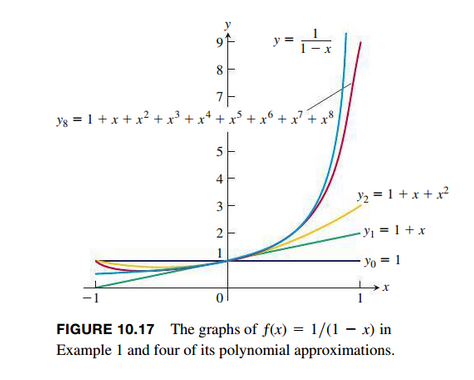
\includegraphics[width = .85\textwidth]{./img/pseriesapprox.png}
\end{center}

Within our image, we can see that the approxmation $ P_{n} ( x )$
improves with the addition of more terms. In the most simple
sense, we are essentially just making the polynomial
derived from the sequence more and more similar to the
graph of the actual function. In this sense, if we were
able to hypothetically add an \textbf{infinite} amount of
terms to the power series, then we would be able to get
an approxmation that is equal to the original function at
some value $ x $.
\begin{remark*}[(2)]
  Find the components of the following series. Then, evaluate
  for what function the series converges to, what the
  radius of convergence is, as well as the infinite sum
  that represents the series.
  \[ 1 - \frac{1}{2}(x-2) + \frac{1}{4} (x-2)^{2} + \cdots
  + \Biggr( -\frac{1}{2}\Biggr)^{n} (x-2)^{n} \]
\end{remark*}

Recall that whenever we are dealing with a power series,
we are trying to think of the terms of the series as
terms within a \textbf{polynomial}. The general form of a
power series is as follows:

\[ \sum_{n=0}^{\infty} c_{n}(x-a)^{n} \]
\[\Rightarrow c_{0} + c_{1}(x-a) + c_{2}(x-a)^{2} +
  c_{3}(x-a)^{3} + \cdots c_{n}(x-a)^{n}\]
Whenever we apply this general structure to the
given power series, we can see that the center $ a $ of the
power series must be 2. Additionally, we can see that
$ c_{0} = 1 $, $c_{1} = - \frac{1}{2}$, $c_{2} = \frac{1}{4}$,
and $ c_{n} = \Biggr( - \frac{1}{2}\Biggr)^{n}$.
Therefore, we are able to translate this power series
to the following infinite sum.

\[ \Rightarrow \sum_{n=0}^{\infty} \Biggr( - \frac{1}{2}  \Biggr)^{n} (x-2)^{n} \]

Because both of the terms of hte power series are
functions of $ n $, then we are able to rewrite the series
in terms of one single ratio $ r$:
\[ \Rightarrow \sum_{n=0}^{\infty} \Biggr( - \frac{(x-2)}{2}  \Biggr)^{n }\]

Given that the infinite sum has the form of a
\textbf{geometric series}, we are able to determien its
\textbf{radius of convergence} knowing that the $ |r| < 1 $.
\[ \Biggr| - \frac{x-2}{2}  \Biggr| < 1 \]
\[ \Rightarrow \Biggr| \frac{x-2}{2}  \Biggr| < 1 \]
\[ \Rightarrow 0 < x < 4 \]
We know that the series will converge only for values of
$ x \in (0,4)$. In order to determine what the series
actually converges to, we are able to apply the
\textbf{sum of a geometric series formula}.
\[ \frac{1}{1-r}\]
\[ \Rightarrow \frac{1}{1+\frac{x-2}{2}}\]
\[ \Rightarrow \frac{2}{2 + x - 2 }\]
\[ \Rightarrow \frac{2}{x}\]
We know that our infinite sum is meant to represent the
function $ f(x) = \frac{2}{x}$ for all values $ x \in (0, 4)$.
The polynomial $ P(n) $, which is equal to the series that
we are given, gives aproximations to the function $ f(x) = \frac{2}{x}$ for any value of $ x $ near 2. From this, we
are able to determine that the following partial sums
\[ P_{0}(x) = 1\]
\[ \Rightarrow  P_{1}(x) = 1 - \frac{1}{2}(x-2)\]
\[ \Rightarrow P_{2}(x) = 1 - \frac{1}{2}(x-2) +
  \frac{1}{4}(x-2)^{2} \]

are just approximations of the function $ \frac{2}{x}$  that
get more and more accurate with the addition of more terms.

Note, though, power series are not just restricted to
geometric series, as we can derive power series (and
approximations of functions with polynomials) with
other types of series.

\section{The Convergence Theorem of Power Series}
Our experiemntation with power series convergence
leads us to the following theorem: \textbf{the Convergence
  Theorem of Power Series}, which offers us a general
idea of how convergence works for power series-- that is,
how we can determine what values of $ x $ the power
series converges to.
\begin{center}
  \fbox{
    \parbox{\textwidth} {
      \begin{thm}
        Convergence Theorem of Power Series
      \end{thm}
      If the power series
      \[ \sum_{n=0}^\infty a_{n}x^{n} =
        a_{0} + a_{1}x + a_{2}x^{2} + a_{3}x^{3} +
        \cdots \]
      converges at $ x = c \neq 0 $, then it
      converges absolutely $ \forall $ such that
      $ |x| < |c| $. If the series diveresg at $ x = d $,
      then it diverges $ \forall $ x such that
      $ | x | > | d | $.
          }
  }
\end{center}
Essentially, this theorem tells us that if we have a
power series that is centered at $ x = 0 $, then if the
series converges at some nonzero value $ c $, then $ x $
will converge for all values within the interval $ - c < x
< c $ and if we know that a power series diverges at $ x = d $,
then the series will diverge for all values of $ x < d $ and
$ x > d $.
\par Note that the theorem does \textit{not} tell us
whether or not that if $ x = c $, then $ c $ is the
\textit{endpoint} of convergence. It merely states that any value
below $ c $ will converge.
\par The other issue with this theorem, though, is that
although it does give us a general idea of the behavior
of a convergent power series, it only offers us informatoin
on the behavior of a convergent power series that is
\textit{centered at $ a = 0 $}. If we want to understand
how power series that are centered at nonzero values
function, then we can look at \textbf{a Corollary to the
  Convergence Theorem of Power Series}. By looking to the
\textbf{corollary of the the convergence theorem to power series},
we are able to describe all \textbf{three possible behaviors} of
power series.

\subsection{Corollary to the Convergence Theorem of Power Series}
\begin{center}
  \fbox{
    \parbox{\textwidth} {
      \begin{definition}
        Corollary to the Convergence Theorem of Power Series
      \end{definition}
      The convergence of the series $ \sum_{n=0}^{\infty} $ is
      described by three of the following behaviors
      \begin{enumerate}
        \item There is some positive number $ R $ such that
              the seires diverges for $ x $ for
              $ x $ with $ | x - a | > R $ but converges
              absolutely for $ x $ with $ | x - a | < R $.
              Series may or may not converge at endpoints $
              x = a- R$ and $ x = a+R$
        \item Converges absolutely $ \forall $ $ x $ (
              this is the situation in which the radius
              $ R =
              \infty $).
        \item Series converges at $ x = a $ and
              diverges $ \forall ~ x \neq a $ ( such
              that the radiu sof convergence is
              $ R = 0 $).
      \end{enumerate}
    }
  }
\end{center}

\subsection{The Three Possible Behaviors of Power Series}
From both the \textbf{convergence theorem of power series} as
well as the \textbf{corollary of the convergence theorem of
  power series}, we can establish that there are three
different types of behaviors of convergent power series.
\begin{enumerate}
  \item $ \sum a_{n} $ converges for $ x = c $ (converges at
        a single point).
  \item $ \sum a_{n} $ converges $ \forall~ x \in (
        -\infty, \infty) $ (converges for all values of $ x $).
  \item $ \sum a_{n} $ converges $ \forall ~ x \in R $,
        such that $ R $ is some interval ( converges for an
        interval).

\end{enumerate}

In the corollary, we discuss the variable $ R $. $ R $
represents the \textit{radius of convergence}, which
represents the distance between the center of the
power series $ a $ from the endpoints of convergence. The
interval of convergence for a power series centered
at $ a $ is as follows:
\[ | x - a | < R \textrm{ or } a - R < x < a + R \]
All values within the interval of convergence
are \textbf{absolutely convergent}, whereas the endpoints
are dpenedent on the series itself. This interval can be
\begin{itemize}
  \item open
  \item closed
  \item or half-open
\end{itemize}
That being said, there is also possibility that the
radius of convergence is \textit{infinite}, which
implies that the series converges for all values of
$ x $, or that the radius of convergence is equal to 0,
which means that the power series only converges at some
value $ x = a $.


\section{Testing Power Series for Convergence}
Here is a computational algorithm for determining where
a power series converges
\begin{center}
  \fbox{
    \parbox{\textwidth} {
      \begin{definition}
        How to Test a Power Series for Convergence
      \end{definition}
      \begin{enumerate}
        \item Use Ratio Test/Root Test to find hte largest
              open interval where the series converges
              absolutely such that
              \[ | x- a | < R ~ \textrm{or }
              a - R < x < a + R \]
        \item If $ R $ is finite, test for convergence
              or divergence \textbf{at each endpoint} by using
              the Comparison Test, Integral Test, or Alternating
              Series Test.
        \item If $ R $ is finite, the series diverges
              for $ | x - a | > R $ (it does not even
              converge conditionally), since the $n$th
              term does not approach zero for those values
              of $ x $.
      \end{enumerate}
          }
  }
\end{center}



\section{Summary of the Behavior of Power Series}
Recall that a power series is just a series that
resembles an \textit{infinite polynomial}. Power
series usually possess some constant $ c_{n}$ as well
as a \textit{center of convergence} $ a $.
\[ \sum_{n=0}^{\infty} c_{n}(x-a)^{n} =
  c_{0} + c_{1}(x-a) + c_{2}(x-a)^{2} + c_{3}(x-a)^{3} + \cdots
+ c_{n}(x-a)^{n}\]
Whenever we are working with power series, it is
important to remember that we aren't necessarily
thinking of the power series as an infinite series,
but rather, an \textit{approximation} of a polynomial.
These polynomials are generally just the point at
which the power series converges, as we can just think of
each term (as well as the terms behind it) as approximations
of this polynomial $ f(x)$. Each approximation $ P_{n}(x)$ improves
with the addition of more terms.
In our examples, we analyzed what forms power series can look
like as well as what it means for a power series to \textbf{converge}. Because power series are an
\textbf{expression} of $ x $, then we have to determine
what values of $ x $ satisfy the series in order to make it
converge. We can determine this by analyzing the archetype
of the power series itself (asking whether or not
it resembles a Ratio Test/Root Test/Geometric Series Test),
and then performing the test, then evaluating the result
of that test for $ x $. We will find that there are
several situations of convergence for a power series,
as the power series can converge at a single value of $ x $,
can converge for an interval of $ -R < x - a < R $ (which
can either be open, closed, or half-open), or can converge
for all values of $ x $. We also analyzed what it means
for a power series to converge and diverge by looking at the
\textbf{Covergence of Power Series Theorem} as well as the
\textbf{Corollary to the Convergence of Power Series Theorem},
which essentially states that if we can determine that a
power series converges for some nonzero value $ c $, then
the series must converge for all values such that $ | x | < c $,
although of course, it doesn't state that $ c $ is necessarily
an endpoint of the interval of convergence. Similarly, we
know that if a power series diverges for a value $ d $, then
the power series will diverge for all values of $ | x | > | d | $.
\par We also generated a general method/ computational algorithm
for determining whether or not a power series converges.
\begin{enumerate}
  \item First, we want to apply the ratio/root test in order
        to evaluate where the given power series
        converges, which is generally in the form of
        \[ | x - a | < R \textrm{ or } a - R < x < a + R \]
  \item Then, we want to determine the activity of the
        power series at the endpoints, since we can only determine
        the \textbf{open interval} of convergence. We can
        determine the behavior of the power series at the
        endpoints by using other convergence tests, such
        as the \textbf{Comparsion Test}, the \textbf{Integral
        Test}, as well as the \textbf{Alternating Series Test}.
  \item We know, however, that all values outside of this
        interval will \textit{always diverge}.
\end{enumerate}


\chapter{10.7 (Part Two): Radius and Interval of Convergence}
\section{Reminders (as of (05/05/23))}
\subsection{MATH\_226}
\begin{enumerate}
  \item  \textbf{Midterm 2} is on \textbf{Tuesday, May 15th, 2023}, which is \textbf{10 days away.}
  \item Remember to revise \textbf{MyLab 15:
        Applications of Taylor Series}.
  \item \textbf{MyLab 16: Complex Numbers} is
        due \textbf{tomorrow, Saturday, May 06, 2023.}
  \item \textbf{Written Homework 7} is due on
        \textbf{Friday, May 12, 2023}.
\end{enumerate}
\subsection{MATH\_230}
\begin{enumerate}
  \item \textbf{230 Midterm 2} is in \textbf{10 days} on
        \textbf{Tuesday, May 15, 2023}.
  \item \textbf{MLM 12: Functions of Multiple Variables} needs revisio n
  \item \textbf{MLM 13: Limits and Continuity in Higher
        Dimensions} is due on \textbf{Sunday, May 7, 2023}.
  \item \textbf{MLM 14: Partial Derivatives} is due on
        \textbf{Tuesday, May 9, 2023.}
        \textbf \textbf{MLM 15: The Chain Rule} is due on
        \textbf{Thursday, May 11, 2023.}
  \item \textbf{WHW 4} is due on \textbf{Wednesday,
        May 10, 2023}.

\end{enumerate}

\section{Motivation}
In the last sectoin, we introduced the idea of the \textbf{power series},
which is essentially just a series that mimics
a \textbf{polynomial} in the form of
\[ \sum_{n=0}^{\infty} c_{n}x^{n} = c_{0} +
c_{1}x + c_{2}x^{2} c_{3}x^{3} + \cdots + c_{n}x^{n}. \]
As we can see, term of of the power series are all
diferentiated by their powers, which allows us to think
of them and treat them \textbf{like polynomials}. In
this new way of htinking, we are no longer thinking of series
as just partial sums, but we're thinking of them as
\textbf{approximations of more interesting functions}.
For example, one of the easitest to remember power series
is the series
\[ \sum_{n=0}^{\infty} \frac{x^{n}}{n!} = 1 + \frac{x}{1!} + \frac{x^{2}}{2!} + \frac{x^{3}}{3!} + \frac{x^{4}}{4!} +
  \cdots + \frac{x^{n}}{n!}\]
This power series is just an estmation of the function
$ e^{x} $, which is also known as the \textbf{exponential
  function}. However, notice that the exponential function
is a function of \textbf{two variables}, $ x $ and $ n $, which
means that there is a \textbf{domain} as well as a \textbf{range} that we are considering whenever we are expanding htis
power seires as well as working with it. In this section,
we are going to be investigating what it means for a
power series to converge, as we can see that if there
is a \textbf{domain} of a power series, is it bounded? If it
is bounded, how do we find these bounds?
\section{Objectives}
\begin{enumerate}
  \item Detemrine whether a power series converges at a point
        by applying convergence tests for infinite series
  \item Determine the radius of convergence of a power
        series.
  \item Completely determine the interval of
        convergence of a power series.
\end{enumerate}

\chapter{10.7 (Part Three): Manipulation of Series (Part One)}
\section{Reminders (as of (05/05/23))}
\subsection{MATH\_226}
\begin{enumerate}
  \item  \textbf{Midterm 2} is on \textbf{Tuesday, May 15th, 2023}, which is \textbf{10 days away.}
  \item Remember to revise \textbf{MyLab 15:
        Applications of Taylor Series}.
  \item \textbf{MyLab 16: Complex Numbers} is
        due \textbf{tomorrow, Saturday, May 06, 2023.}
  \item \textbf{Written Homework 7} is due on
        \textbf{Friday, May 12, 2023}.
\end{enumerate}
\subsection{MATH\_230}
\begin{enumerate}
  \item \textbf{230 Midterm 2} is in \textbf{10 days} on
        \textbf{Tuesday, May 15, 2023}.
  \item \textbf{MLM 12: Functions of Multiple Variables} needs revisio n
  \item \textbf{MLM 13: Limits and Continuity in Higher
        Dimensions} is due on \textbf{Sunday, May 7, 2023}.
  \item \textbf{MLM 14: Partial Derivatives} is due on
        \textbf{Tuesday, May 9, 2023.}
        \textbf \textbf{MLM 15: The Chain Rule} is due on
        \textbf{Thursday, May 11, 2023.}
  \item \textbf{WHW 4} is due on \textbf{Wednesday,
        May 10, 2023}.

\end{enumerate}

\section{Objectives}
\begin{enumerate}
  \item Multiply, differentiate, and integrate
        convergent power series
  \item Compose a convergent power series with a
        monomial function to generate a new convergent
        power series
  \item Compute power series representation sof
        elementary functions by manipulating known
        power series.
\end{enumerate}

\section{Motivation}
In the former section, we exposed ourselves to the
world of \textbf{power series}, which are infinite series
that resemble ``infinite polynomials'', meaning that
we have an infinite number of terms of varying
exponential degrees. Power series generally come in the
general form
\[ \sum_{n=0}^{\infty} c_{n} (x-a)^{n} =
  c_{0} + c_{1}(x-a) + c_{2}(x-a)^{2} + c_{3}(x-a)^{3} +
  \cdots + c_{n}(x-a)^{n}\]
such that $ c_{n}$ is just a constant and $ a $ is known
as the \textit{center of the interval of convergence}.
We saw that the terms of the power series are interesting
because they are able to represent \textit{approximations} of
functions $ f(x)$. We have observed that these approximations,
which represent the first $n$ terms of a power series $ P_{n}(x)$
beocme more accurate as we include more terms.
\par Finally, we observed the behavior of convergence
and divergence within power series. We saw that because
power series are multivariable expressions of $ x $ and $ n $,
that they are able to converge across numerous values of $ x $.
We observed that we can apply different \textit{convergence
  tests}, such as the Geometric Series Test, the Ratio Test,
as well as the Root Test in order to determine whether or not
a given power series converges, and, more importantly,
\textit{where} the given power series converges. Once
we determine where the power series converges, which is
an open interval, we then have to determine the behavior of the
power series at the endpoints of this interval, which we
can assess using more convergence tests such as the
Comparison Test, the Integral Test, as well as the Alternating
Series Test.

Now that we have the basic principles of power series (suggesting
what they are as well as their different behavior), let us
now observe methods of which we are able to \textit{manipulate
  power series} and work with them. In the previous section,
we have alluded to adding, subtracting, multiplying, differentiating, and even integrating power series, and in this
section, we are learning how to do this.

\section{Operations on Power Series}
We are able to perform numerous algebraic operatoins
on two given power series. However, of course, this means
that we are performing these operations on the
\textbf{intersections of the two series' intervals of
  convergence}. Again, since we are merely just thinking
of these series as polynomials, we can apply
our intuition of operations on polynomials to operations
of power series.
\begin{enumerate}
  \item We multiply power series by distributing each term,
        much like FOILing
  \item We add power series by adding like terms
  \item We subtract power series by subtracting like
        terms
  \item We divide power series similarly to as
        we divide two polynomials
\end{enumerate}

\begin{center}
  \fbox{
    \parbox{\textwidth} {
      \begin{definition}
        Series Multiplication for Power Series
      \end{definition}
      If $ A(x) = \sum_{n=0}^{\infty} a_{n}x^{n}$ and $ B(x) =
      \sum_{n=0}^{\infty} b_{n}x^{n }$ converge absolutely
      for $ | x | < R$, and
      \[ c_{n} = a_{0}b_{n} +
        a_{1}b_{n-1} + a_{2}b_{n-2} + \cdots
        a_{n-1}b_{1} + a_{n}b_{0} = \sum_{n=0}^{\infty} a_{k}b_{n-k}, \]
      then $ \sum_{n=0}^{\infty} c_{n}x^{n}$ converges
      absolutely to $ A(x) \cdot B(x) $ for $ |x| < R $
      \[ \Biggr( \sum_{n=0}^{\infty} a_{n}x^{n}   \Biggr) \cdot \Biggr( \sum_{n=0}^{\infty} b_{n}x^{n}  \Biggr)\]
      Evidently, it is a little tricky to find the
      coefficient of the resulting series $ c_{n} $, since
      it requires us to \textit{manually mutliply the terms
      and determine a general pattern}.
    }
  }
\end{center}

\begin{remark*}[1]
  Multiply the power series
  \[ \sum_{n=0}^{\infty} x_{n} \textrm{ and } \sum_{n=0}^{\infty}
  (-1)^{n} \frac{x^{n+1}}{n+1} \]
\end{remark*}
\begin{center}
  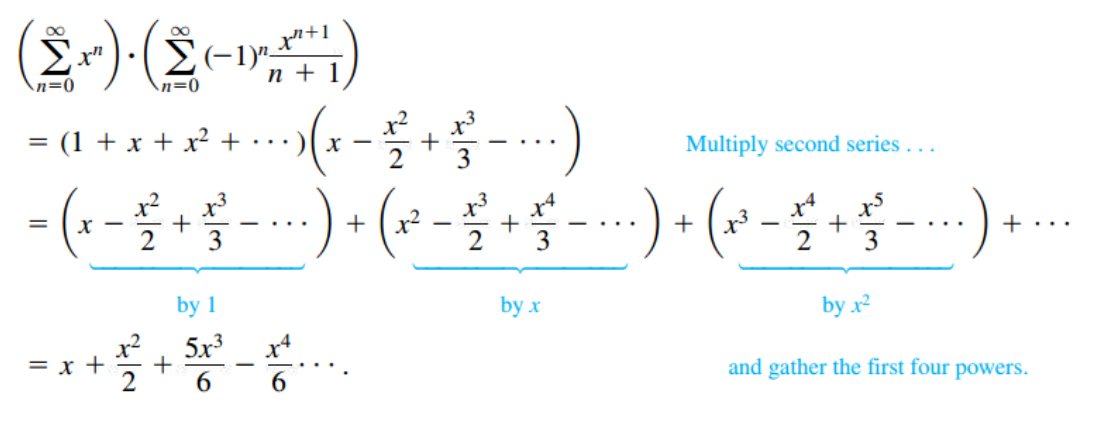
\includegraphics[width = 0.95\textwidth]{./img/thm19ex.png}

\end{center}

\section{Substituting Functions into Convergent Power Series}
Much as we are able to multiply power series within
their overlapping intervals of convergence,
we are also able to substitute functions whose values are
within the interval of convergence $ |f(x)| < R $ into
different power series.

\begin{center}
  \fbox{
    \parbox{\textwidth} {
      \begin{definition}
        Theorem 20 (Subsituting Functions into Power
        Series)
      \end{definition}
      If $ \sum_{n=0}^{\infty} a_{n}x^{n}$ converges
      absolutely for $ |x| < R $ and $ f $ is a continuous
      function, then $ \sum_{n=0}^{\infty} a_{n}(f(x))^{n}$
      converges absolutely on the set of points
      $ x $such that the range of the function $ f(x)$
      is within the radius of convergence, or $ |f(x)| < R $.
    }
  }
\end{center}

\begin{remark*}[(2) Substituting Functions into Power Series]
  Determine the interval of convergence for the following
  power series only using subsitution.
  \[ \sum_{n=0}^{\infty} (4x^{2})^{n}\]
\end{remark*}
Whenever we are approaching this problem, we can observe
what we do know. In the former section, we observed that the
power series
\[ \sum_{n=0}^{\infty} x^{n} \]
will converge for all values of $ |x| < 1 $, since we
are able to think of the power series as a geometric series.
We know that the power series, in this specific case,
will converge to the value
\[ \frac{1}{1-x}\]
Since we know that the function $ 4x^{2}$ is continuous,
then we are able to substitute $ x $ for $ 4x^{2}$, and see
that power series represents the function
\[ \frac{1}{1-4x^{2}}\] and, most importantly,
will converge for the expression $ |x| < 1 \to |4x^{2}| < 1 $.
From evaluating the inequality, we observe that the power series $ \sum_{n=0}^{\infty} (4x^{2})^{n}$
will converge at $ |x| < \frac{1}{2}$.

In addition to being able to add power series, mulitply
power series, and even substitute functions into power series,
we are also able to \textbf{differentiate power series term by term
for all values of $ x $ within their interval of convergence}.

\subsection{Term-By-Term Differentation of Power Series}
\begin{center}
  \fbox{
    \parbox{\textwidth} {
      \begin{definition}
        (Theorem 21) Term-By-Term Differentiation
      \end{definition}
      If $ \sum c_{n}(x-a)^{n} $has the radius of convergence
      $ R > 0 $, it defines a function
      \[ f(x) = \sum_{n=0}^{\infty} c_{n}(x-a)^{n} \textrm{ on the interval }
        a - R < x < a + R \]
      This function $ f $ has derivatives of all orders inside the interval, and we
      obtain the derivatives by differentiating the original series term by term. Here
      are the derivatives of a power series.
      \[ f'(x) = \sum_{n=1}^{\infty} nc_{n}(x-a)^{n-1}\]
      \[ f''(x) = \sum_{n=2}^{\infty} n(n-1)c_{n}(x-a)^{n-2}\]
      and so on. Each of these derived series converges at every point of the
      interval $ a - R < x < a +R $, which is consistent between
      \textit{all derivatives}.
    }
  }
\end{center}
Essentially, we are able to find the \textbf{derivatives} of terms within
a power series that are within the interval of convergence of that power series. We
find the derivatives of the power series (that is, the expression that defines
the power series) by literally finding the derivatives of each term and generating
a new power series expression from it.
\par \textbf{Note:} Whenever we are evaluating the derivative of a
power series, note how we change the \textbf{starting index}.
The reason that this is, is that, whenever we actually derive the power series,
the resulting function will always have an exponent of $ n - a $, such that
a is just some number. This means that at $ n =0 $, the initial term will
always be zero. Therefore, we just reindex the derivative of hte power series
in order to avoid this initial zero.
\par \textbf{Note:} Term-by-term differentation does not work for \textit{all}
power series. For example, if we use the trigonometric series
\[ \sum_{n=0}^{\infty} \frac{sin(n!x)}{n^{2}}  \]
converges for all $ x $. But if we differentaite term by term
we obtain the following series
\[ \sum_{n=1}^{\infty} \frac{n!\cos{n!x}}{n^{2}} \]
which diverges for all $ x $. Note how these two series are \textbf{not}
power series, since they are not a sum of \textit{positive integer powers of $x$ }.
\\ \\
In addition to being able to differentiate a power series, we are also able to
\textit{integrate} a power series and find antiderivatives that exist on
the same interval of convergence.

\subsection{Term-By-Term Integration}
\begin{center}
  \fbox{
    \parbox{\textwidth} {
      \begin{definition}
        (Theorem 22) Term-By-Term Integration

      \end{definition}
      Suppose that
      \[ f(x) = \sum_{n=0}^{\infty} c_{n}(x-a)^{n} \]
      converges for $ a - R < x < a + R (R > 0) $. Then
      \[ \sum_{n=0}^{\infty} c_{n} \frac{(x-a)^{n+1}}{n+1}\]
      converges for $ a - R < x < a + R (R > 0) $ and
      \[ \int_{}^{} f(x)dx =  \sum_{n=0}^{\infty} c_{n} \frac{(x-a)^{n+1}}{n+1} + C \]
      for $ a - R < x < a + R $.
    }
  }
\end{center}
  The consequences of being able to manipualte series like this is that
  we're able to find sequences that have the same exact radius of
  convergence, which allows us to discover functions that
  behave in similar ways (although, of course, not
  in the same exact way). In the given examples, we
  differentiate and integrate power series, starting with
  a power series, then integrating it, only to find it
  to resemble a more familar power series of which
  we know the point of convergence (or the fucntino that
  the power series represents), and then we can just
  integrate that function to find what the original
  power series represents.
  \par It is important to understand that whenever
  we are integrating a power series, we are
  literally integrating all of the terms of
  the power series, similarly to how when
  we differentiate a power series, we are
  literally differentiating all of the terms
  of the power series. We are obtianing
  a series that, although is not going
  to yield the same sum as the original
  function, will behave similarly to the
  original function, albeit with different
  centers, for example. It is important
  for us to be able to freely differentiate
  and integrate series as well as multiply and
  divide them.
  The general form for differentiation and
  integration is as follows
  \[ \frac{d}{dx} \sum_{n=0}^{\infty} c_{n}x^{n} = nc_{n}x^{n-1}\]
  \[ \frac{d^{2}}{dx^{2}} \sum_{n=0}^{\infty} c_{n}x^{n} = (n-1)nc_{n}x^{n-2}\]
  As for integration:
  \[ \int c_{n}(x-a)^{n} dx  = \sum_{n=0}^{\infty} c_{n} \frac{(x-a)^{n+1}}{n+1} + C \]

\chapter{10.7 (Part Four): Manipulation of Series (Part Two)}
\section{Reminders (as of (05/05/23))}
\subsection{MATH\_226}
\begin{enumerate}
  \item  \textbf{Midterm 2} is on \textbf{Tuesday, May 15th, 2023}, which is \textbf{10 days away.}
  \item Remember to revise \textbf{MyLab 15:
        Applications of Taylor Series}.
  \item \textbf{MyLab 16: Complex Numbers} is
        due \textbf{tomorrow, Saturday, May 06, 2023.}
  \item \textbf{Written Homework 7} is due on
        \textbf{Friday, May 12, 2023}.
\end{enumerate}
\subsection{MATH\_230}
\begin{enumerate}
  \item \textbf{230 Midterm 2} is in \textbf{10 days} on
        \textbf{Tuesday, May 15, 2023}.
  \item \textbf{MLM 12: Functions of Multiple Variables} needs revisio n
  \item \textbf{MLM 13: Limits and Continuity in Higher
        Dimensions} is due on \textbf{Sunday, May 7, 2023}.
  \item \textbf{MLM 14: Partial Derivatives} is due on
        \textbf{Tuesday, May 9, 2023.}
        \textbf \textbf{MLM 15: The Chain Rule} is due on
        \textbf{Thursday, May 11, 2023.}
  \item \textbf{WHW 4} is due on \textbf{Wednesday,
        May 10, 2023}.

\end{enumerate}


\section{Objectives}
\begin{enumerate}
  \item Multiply, differentiate, and integrate convergent
        power series
  \item Compose a convergent power series with a
        monomial function to generate new power series
  \item Compute power series rperesentations of several
        elementary functions by manipualting known
        convergent power series
  \item Explain the connection between the coefficients
        of a power series and the sum of a power series
\end{enumerate}

\section{Motivation}
\chapter{10.8 (Part One): Taylor Series}
\section{Reminders (as of (05/05/23))}
\subsection{MATH\_226}
\begin{enumerate}
  \item  \textbf{Midterm 2} is on \textbf{Tuesday, May 15th, 2023}, which is \textbf{10 days away.}
  \item Remember to revise \textbf{MyLab 15:
        Applications of Taylor Series}.
  \item \textbf{MyLab 16: Complex Numbers} is
        due \textbf{tomorrow, Saturday, May 06, 2023.}
  \item \textbf{Written Homework 7} is due on
        \textbf{Friday, May 12, 2023}.
\end{enumerate}
\subsection{MATH\_230}
\begin{enumerate}
  \item \textbf{230 Midterm 2} is in \textbf{10 days} on
        \textbf{Tuesday, May 15, 2023}.
  \item \textbf{MLM 12: Functions of Multiple Variables} needs revisio n
  \item \textbf{MLM 13: Limits and Continuity in Higher
        Dimensions} is due on \textbf{Sunday, May 7, 2023}.
  \item \textbf{MLM 14: Partial Derivatives} is due on
        \textbf{Tuesday, May 9, 2023.}
        \textbf \textbf{MLM 15: The Chain Rule} is due on
        \textbf{Thursday, May 11, 2023.}
  \item \textbf{WHW 4} is due on \textbf{Wednesday,
        May 10, 2023}.

\end{enumerate}

\section{Objectives}
\begin{enumerate}
  \item Compute the Taylor (as well as MacLaurin) seires
        generated by an infinitely differentiable
        fucntion centered at a given point.
  \item Explore the relationships between the
        coefficient sof a power series and the sum of the
        same power series
\end{enumerate}

\section{Motivation}
\chapter{10.8 (Part Two): Taylor Polynomials and
Taylor Series Convergence }
\section{Reminders (as of (05/05/23))}
\subsection{MATH\_226}
\begin{enumerate}
  \item  \textbf{Midterm 2} is on \textbf{Tuesday, May 15th, 2023}, which is \textbf{10 days away.}
  \item Remember to revise \textbf{MyLab 15:
        Applications of Taylor Series}.
  \item \textbf{MyLab 16: Complex Numbers} is
        due \textbf{tomorrow, Saturday, May 06, 2023.}
  \item \textbf{Written Homework 7} is due on
        \textbf{Friday, May 12, 2023}.
\end{enumerate}
\subsection{MATH\_230}
\begin{enumerate}
  \item \textbf{230 Midterm 2} is in \textbf{10 days} on
        \textbf{Tuesday, May 15, 2023}.
  \item \textbf{MLM 12: Functions \section{Reminders (as of (05/05/23))}
\subsection{MATH\_226}
\begin{enumerate}
  \item  \textbf{Midterm 2} is on \textbf{Tuesday, May 15th, 2023}, which is \textbf{10 days away.}
  \item Remember to revise \textbf{MyLab 15:
        Applications of Taylor Series}.
  \item \textbf{MyLab 16: Complex Numbers} is
        due \textbf{tomorrow, Saturday, May 06, 2023.}
  \item \textbf{Written Homework 7} is due on
        \textbf{Friday, May 12, 2023}.
\end{enumerate}
\subsection{MATH\_230}
\begin{enumerate}
  \item \textbf{230 Midterm 2} is in \textbf{10 days} on
        \textbf{Tuesday, May 15, 2023}.
  \item \textbf{MLM 12: Functions of Multiple Variables} needs revisio n
  \item \textbf{MLM 13: Limits and Continuity in Higher
        Dimensions} is due on \textbf{Sunday, May 7, 2023}.
  \item \textbf{MLM 14: Partial Derivatives} is due on
        \textbf{Tuesday, May 9, 2023.}
        \textbf \textbf{MLM 15: The Chain Rule} is due on
        \textbf{Thursday, May 11, 2023.}
  \item \textbf{WHW 4} is due on \textbf{Wednesday,
        May 10, 2023}.

\end{enumerate}

\section{Motivation}of Multiple Variables} needs revisio n
  \item \textbf{MLM 13: Limits and Continuity in Higher
        Dimensions} is due on \textbf{Sunday, May 7, 2023}.
  \item \textbf{MLM 14: Partial Derivatives} is due on
        \textbf{Tuesday, May 9, 2023.}
        \textbf \textbf{MLM 15: The Chain Rule} is due on
        \textbf{Thursday, May 11, 2023.}
  \item \textbf{WHW 4} is due on \textbf{Wednesday,
        May 10, 2023}.

\end{enumerate}

\section{Motivation}
\section{Reminders (as of (05/05/23))}
\subsection{MATH\_226}
\begin{enumerate}
  \item  \textbf{Midterm 2} is on \textbf{Tuesday, May 15th, 2023}, which is \textbf{10 days away.}
  \item Remember to revise \textbf{MyLab 15:
        Applications of Taylor Series}.
  \item \textbf{MyLab 16: Complex Numbers} is
        due \textbf{tomorrow, Saturday, May 06, 2023.}
  \item \textbf{Written Homework 7} is due on
        \textbf{Friday, May 12, 2023}.
\end{enumerate}
\subsection{MATH\_230}
\begin{enumerate}
  \item \textbf{230 Midterm 2} is in \textbf{10 days} on
        \textbf{Tuesday, May 15, 2023}.
  \item \textbf{MLM 12: Functions of Multiple Variables} needs revisio n
  \item \textbf{MLM 13: Limits and Continuity in Higher
        Dimensions} is due on \textbf{Sunday, May 7, 2023}.
  \item \textbf{MLM 14: Partial Derivatives} is due on
        \textbf{Tuesday, May 9, 2023.}
        \textbf \textbf{MLM 15: The Chain Rule} is due on
        \textbf{Thursday, May 11, 2023.}
  \item \textbf{WHW 4} is due on \textbf{Wednesday,
        May 10, 2023}.

\end{enumerate}

\section{Motivation}

\chapter{Convergence of Taylor Series ((05/05/23))}
\section{Reminders (as of (05/05/23))}
\subsection{MATH\_226}
\begin{enumerate}
  \item  \textbf{Midterm 2} is on \textbf{Tuesday, May 15th, 2023}, which is \textbf{10 days away.}
  \item Remember to revise \textbf{MyLab 15:
        Applications of Taylor Series}.
  \item \textbf{MyLab 16: Complex Numbers} is
        due \textbf{tomorrow, Saturday, May 06, 2023.}
  \item \textbf{Written Homework 7} is due on
        \textbf{Friday, May 12, 2023}.
\end{enumerate}
\subsection{MATH\_230}
\begin{enumerate}
  \item \textbf{230 Midterm 2} is in \textbf{10 days} on
        \textbf{Tuesday, May 15, 2023}.
  \item \textbf{MLM 12: Functions of Multiple Variables} needs revisio n
  \item \textbf{MLM 13: Limits and Continuity in Higher
        Dimensions} is due on \textbf{Sunday, May 7, 2023}.
  \item \textbf{MLM 14: Partial Derivatives} is due on
        \textbf{Tuesday, May 9, 2023.}
        \textbf \textbf{MLM 15: The Chain Rule} is due on
        \textbf{Thursday, May 11, 2023.}
  \item \textbf{WHW 4} is due on \textbf{Wednesday,
        May 10, 2023}.

\end{enumerate}

\section{Motivation}

\chapter{Applications of Taylor Series}
\section{Reminders (as of (05/05/23))}
\subsection{MATH\_226}
\begin{enumerate}
  \item  \textbf{Midterm 2} is on \textbf{Tuesday, May 15th, 2023}, which is \textbf{10 days away.}
  \item Remember to revise \textbf{MyLab 15:
        Applications of Taylor Series}.
  \item \textbf{MyLab 16: Complex Numbers} is
        due \textbf{tomorrow, Saturday, May 06, 2023.}
  \item \textbf{Written Homework 7} is due on
        \textbf{Friday, May 12, 2023}.
\end{enumerate}
\subsection{MATH\_230}
\begin{enumerate}
  \item \textbf{230 Midterm 2} is in \textbf{10 days} on
        \textbf{Tuesday, May 15, 2023}.
  \item \textbf{MLM 12: Functions of Multiple Variables} needs revisio n
  \item \textbf{MLM 13: Limits and Continuity in Higher
        Dimensions} is due on \textbf{Sunday, May 7, 2023}.
  \item \textbf{MLM \section{Reminders (as of (05/05/23))}
\subsection{MATH\_226}
\begin{enumerate}
  \item  \textbf{Midterm 2} is on \textbf{Tuesday, May 15th, 2023}, which is \textbf{10 days away.}
  \item Remember to revise \textbf{MyLab 15:
        Applications of Taylor Series}.
  \item \textbf{MyLab 16: Complex Numbers} is
        due \textbf{tomorrow, Saturday, May 06, 2023.}
  \item \textbf{Written Homework 7} is due on
        \textbf{Friday, May 12, 2023}.
\end{enumerate}
\subsection{MATH\_230}
\begin{enumerate}
  \item \textbf{230 Midterm 2} is in \textbf{10 days} on
        \textbf{Tuesday, May 15, 2023}.
  \item \textbf{MLM 12: Functions of Multiple Variables} needs revisio n
  \item \textbf{MLM 13: Limits and Continuity in Higher
        Dimensions} is due on \textbf{Sunday, May 7, 2023}.
  \item \textbf{MLM 14: Partial Derivatives} is due on
        \textbf{Tuesday, May 9, 2023.}
        \textbf \textbf{MLM 15: The Chain Rule} is due on
        \textbf{Thursday, May 11, 2023.}
  \item \textbf{WHW 4} is due on \textbf{Wednesday,
        May 10, 2023}.

\end{enumerate}

\section{Motivation}14: Partial Derivatives} is due on
        \textbf{Tuesday, May 9, 2023.}
        \textbf \textbf{MLM 15: The Chain Rule} is due on
        \textbf{Thursday, May 11, 2023.}
  \item \textbf{WHW 4} is due on \textbf{Wednesday,
        May 10, 2023}.

\end{enumerate}

\section{Objectives}
\begin{enumerate}
  \item Explore advanced application sof Taylor
        Series representations to major topics in
        single-variable calculus
\end{enumerate}

\section{Motivation}
\chapter{A7 (Part One): Complex Numbers (Part One)}
\section{Reminders (as of (05/05/23))}
\subsection{MATH\_226}
\begin{enumerate}
  \item  \textbf{Midterm 2} is on \textbf{Tuesday, May 15th, 2023}, which is \textbf{10 days away.}
  \item Remember to revise \textbf{MyLab 15:
        Applications of Taylor Series}.
  \item \textbf{MyLab 16: Complex Numbers} is
        due \textbf{tomorrow, Saturday, May 06, 2023.}
  \item \textbf{Written Homework 7} is due on
        \textbf{Friday, May 12, 2023}.
\end{enumerate}
\subsection{MATH\_230}
\begin{enumerate}
  \item \textbf{230 Midterm 2} is in \textbf{10 days} on
        \textbf{Tuesday, May 15, 2023}.
  \item \textbf{MLM 12: Functions of Multiple Variables} needs revisio n
  \item \textbf{MLM 13: Limits and Continuity in Higher
        Dimensions} is due on \textbf{Sunday, May 7, 2023}.
  \item \textbf{MLM 14: Partial Derivatives} is due on
        \textbf{Tuesday, May 9, 2023.}
        \textbf \textbf{MLM 15: The Chain Rule} is due on
        \textbf{Thursday, May 11, 2023.}
  \item \textbf{WHW 4} is due on \textbf{Wednesday,
        May 10, 2023}.

\end{enumerate}

\section{Objectives}
\begin{enumerate}
  \item Explain the significance of the complex number
        systems via the \textbf{Fundamental Theorem of
        Calcuslu}.
  \item Compute the complex conjugate and absolute
        value of a ocmplex number
  \item Algebraically manipulate algebraic expressions
        involving complex numbers
\end{enumerate}

\section{Motivation}
\chapter{10.10, A7 (Part Two): Complex Numbers (Part Two)}
\section{Reminders (as of (05/05/23))}
\subsection{MATH\_226}
\begin{enumerate}
  \item  \textbf{Midterm 2} is on \textbf{Tuesday, May 15th, 2023}, which is \textbf{10 days away.}
  \item Remember to revise \textbf{MyLab 15:
        Applications of Taylor Series}.
  \item \textbf{MyLab 16: Complex Numbers} is
        due \textbf{tomorrow, Saturday, May 06, 2023.}
  \item \textbf{Written Homework 7} is due on
        \textbf{Friday, May 12, 2023}.
\end{enumerate}
\subsection{MATH\_230}
\begin{enumerate}
  \item \textbf{230 Midterm 2} is in \textbf{10 days} on
        \textbf{Tuesday, May 15, 2023}.
  \item \textbf{MLM 12: Functions of Multiple Variables} needs revisio n
  \item \textbf{MLM 13: Limits and Continuity in Higher
        Dimensions} is due on \textbf{Sunday, May 7, 2023}.aaaa
  \item \textbf{MLM 14: Partial Derivatives} is due on
        \textbf{Tuesday, May 9, 2023.}
        \textbf \textbf{MLM 15: The Chain Rule} is due on
        \textbf{Thursday, May 11, 2023.}
  \item \textbf{WHW 4} is due on \textbf{Wednesday,
        May 10, 2023}.

\end{enumerate}

\section{Objectives}
\begin{enumerate}
  \item Understand Euler's fomrula and the polar coordinate
        representations of complex numbers
  \item Be able to visualize the ocmplex plane as
        well as points and expressions of the ocmplex plane
  \item Be able to manipulate the exponential function
        and investigate its propertie sin reltaion to
        complex numbers
        \item Establish roots of unity and \textbf{DeMoivre numbers and theoerems}.

\end{enumerate}

\section{Motivation}
\chapter{19.1 (Part One): Vectors}
\section{Reminders}
\section{Motivation}
\chapter{19.1 (Part Two): Inner Products}
\section{Reminders}
\section{Motivation}

%%%%%%%%%%%% MIDTERM 2 DONE %%%%%%%%%%%%%%%%%%%%%%%%%

\chapter{19.2 (Part One): Functions as Vectors, Periodic
  Functions}
\section{Reminders}
\section{Motivation}
\chapter{19.2 (Part Two): Fourier Series, Demos}
\section{Reminders}
\section{Motivation}
\chapter{19.3: Fourier Series, Theory}
\section{Reminders}
\section{Motivation}
\chapter{19.5 (Part One): Applications (Part One)}
\section{Reminders}
\subsection{MATH\_226}
\begin{enumerate}
  \item \textbf{Written Homework 9: Second-Order Linear Differential Equations} is due on \textbf{Friday, 26, 2023}.
\end{enumerate}

\subsection{MATH\_230}
\begin{enumerate}
  \item \textbf{Written Homework 5} is due on \textbf{
        Wednesday, May 24, 2023}.
  \item \textbf{MyLab Math 17: Tangent Planes
        and Linearization} is due \textbf{tomorrow,
        May 23, 2023}.
  \item \textbf{MyLab Math 18: Taylor's Formula
        } is due \textbf{tomorrow May 23, 2023}.
\end{enumerate}

\section{Motivation}
Throughout the entire ocurse, we have touched
on sequences, series, and how to use them in numerous
different contexts, such as Fourier Series. Now,
however, we want to take our series manipulations
in another direction. For exapmle, what if
we want to approximate the temperature, while
considering all possible conditions?

\section{Brief Introduction to Differntial Equations (17.1)}
\dfn{Second-Order Linear Differential Equations}{
  A \textbf{second-order linear differential equation} is an equation that involves a function $y(x)$ as
  well as its derivatives, usually taking on the
  following form
  \begin{equation}\label{eq1}
    P(x)y''(x) + Q(x)y'(x) + R(x)y(x) = G(x)
  \end{equation}

  There are two different types of second-order
  linear differential equations:
\begin{itemize}
  \item Homogeneous Linear Differential Equations
  \item Heterogeneous Linear Differential
        Equations
\end{itemize}
}

\dfn{Homogeneous Linear Differential Equations}{
  Given the equation \eqref{eq1}, a \textbf{homogeneous linear differential equation} is an equation
  in which $ G(x)$ is equal to zero for all
  values of $ x$ over an interval $ I $.
  This results in the following differential equation
  \begin{equation}\label{eq2}
    P(x)y''(x) + Q(x)y'(x) + R(x)y(x) = 0
  \end{equation}}
\dfn{Heterogeneous Linear Differential Equations}{
  By contrast, a \textbf{heterogeneous linear differential
    equation } is one in which $G(x) \neq 0$ for
  all values of $ x $ over an interval $ I $.}

\section{Evaluating Differential Equations with Power Series (17.5)}
Among the numerous ways we are able to evaluate
differential equatoins, we can actually apply
our familiarity with \textbf{power series} in order
to evaluate differential equations.


\chapter{19.5 (Part Two): Applications (Part Two)}
\section{Reminders}
\section{Motivation}
\end{sloppypar}

\end{document}
